\documentclass[conference,a4paper]{IEEEtran}
\IEEEoverridecommandlockouts
\usepackage{amsmath,amssymb}
\usepackage{graphicx}
\usepackage{multirow}
\usepackage{url}
\usepackage[hidelinks,bookmarks=false]{hyperref}
\hypersetup{pdftitle={Conservative Road-Scene Risk Assessment via Fail-Aware Multi-Model Fusion},
  pdfauthor={Pham Hoang Bach, Vu Gia Tien, Trinh Quang Tien, Cao Van Mai}}
% Generated by camera_ready/paper_numbers.py from results.json. Do not edit.
\newcommand{\HardImages}{100}
\newcommand{\HardAccepted}{505}
\newcommand{\HardStable}{437}
\newcommand{\HardCheck}{67}
\newcommand{\HardUncertain}{1}
\newcommand{\HardStablePct}{86.5}
\newcommand{\HardStableLow}{83.3}
\newcommand{\HardStableHigh}{89.2}
\newcommand{\HardStableBootLow}{83.5}
\newcommand{\HardStableBootHigh}{89.2}
\newcommand{\HardPrec}{86.3}
\newcommand{\HardPrecLow}{82.9}
\newcommand{\HardPrecHigh}{89.6}
\newcommand{\HardRecRel}{72.2}
\newcommand{\HardRecRelLow}{67.2}
\newcommand{\HardRecRelHigh}{77.3}
\newcommand{\HardRecAll}{52.8}
\newcommand{\HardRecAllLow}{47.8}
\newcommand{\HardRecAllHigh}{57.4}
\newcommand{\HardRawPrec}{81.5}
\newcommand{\HardRawRecRel}{77.0}
\newcommand{\HardPathPrec}{15.8}
\newcommand{\HardPathPrecK}{25}
\newcommand{\HardPathPrecN}{158}
\newcommand{\HardPathRec}{56.8}
\newcommand{\HardPathRecK}{25}
\newcommand{\HardPathRecN}{44}
\newcommand{\HardPathOff}{131}
\newcommand{\HardSideDirect}{19}
\newcommand{\HardCorridorIoU}{0.24}
\newcommand{\HardRoadIoU}{0.82}
\newcommand{\HardOccupied}{30}
\newcommand{\HardUnsafe}{0}
\newcommand{\HardUnsafeHigh}{11.4}
\newcommand{\HardUnsafeNoFB}{1}
\newcommand{\HardFree}{67}
\newcommand{\HardOver}{34}
\newcommand{\HardOverPct}{50.7}
\newcommand{\HardSevere}{47}
\newcommand{\HardSeverePct}{47.0}
\newcommand{\HardUnsupported}{31}
\newcommand{\HardUnsupportedPct}{66.0}
\newcommand{\HardEmpty}{15}
\newcommand{\HardFallback}{15}
\newcommand{\HardStop}{5}
\newcommand{\HardBrake}{42}
\newcommand{\HardClear}{1}
\newcommand{\HardClearPct}{1.0}
\newcommand{\HardMonitorPct}{35.0}
\newcommand{\HardFPStable}{11.9}
\newcommand{\HardFPStableLow}{8.9}
\newcommand{\HardFPStableHigh}{15.1}
\newcommand{\HardFPNonStable}{25.0}
\newcommand{\HardFPNonStableLow}{14.5}
\newcommand{\HardFPNonStableHigh}{35.3}
\newcommand{\HardFPRatio}{2.1}
\newcommand{\HardTruncStable}{2.1}
\newcommand{\HardOcclStable}{58.7}
\newcommand{\HardIoUStable}{0.81}
\newcommand{\HardTruncCheck}{78.4}
\newcommand{\HardOcclCheck}{33.3}
\newcommand{\HardIoUCheck}{0.86}
\newcommand{\HardWClearImages}{56}
\newcommand{\HardWClearRecRel}{65.8}
\newcommand{\HardWClearPrec}{81.3}
\newcommand{\HardWClearStablePct}{85.5}
\newcommand{\HardWClearUnsafe}{0}
\newcommand{\HardWClearOccupied}{15}
\newcommand{\HardWClearDegraded}{89}
\newcommand{\HardWClearDayImages}{5}
\newcommand{\HardWClearDayRecRel}{68.8}
\newcommand{\HardWClearNightImages}{50}
\newcommand{\HardWClearNightRecRel}{64.7}
\newcommand{\HardWClearNightPct}{89}
\newcommand{\HardWRainyImages}{8}
\newcommand{\HardWRainyRecRel}{82.9}
\newcommand{\HardWRainyPrec}{90.0}
\newcommand{\HardWRainyStablePct}{82.0}
\newcommand{\HardWRainyUnsafe}{0}
\newcommand{\HardWRainyOccupied}{0}
\newcommand{\HardWRainyDegraded}{25}
\newcommand{\HardWRainyDayImages}{6}
\newcommand{\HardWRainyDayRecRel}{82.5}
\newcommand{\HardWRainyNightImages}{2}
\newcommand{\HardWRainyNightRecRel}{100.0}
\newcommand{\HardWRainyNightPct}{25}
\newcommand{\HardWSnowyImages}{9}
\newcommand{\HardWSnowyRecRel}{85.4}
\newcommand{\HardWSnowyPrec}{94.5}
\newcommand{\HardWSnowyStablePct}{87.3}
\newcommand{\HardWSnowyUnsafe}{0}
\newcommand{\HardWSnowyOccupied}{4}
\newcommand{\HardWSnowyDegraded}{33}
\newcommand{\HardWSnowyDayImages}{6}
\newcommand{\HardWSnowyDayRecRel}{84.8}
\newcommand{\HardWSnowyNightImages}{3}
\newcommand{\HardWSnowyNightRecRel}{100.0}
\newcommand{\HardWSnowyNightPct}{33}
\newcommand{\HardDayImages}{38}
\newcommand{\HardDayStablePct}{87.9}
\newcommand{\HardDayPrec}{91.4}
\newcommand{\HardDayRecRel}{78.1}
\newcommand{\HardDayUnsafe}{0}
\newcommand{\HardDayOccupied}{18}
\newcommand{\HardDayCorridorIoU}{0.20}
\newcommand{\HardDayRoadIoU}{0.81}
\newcommand{\HardNightImages}{60}
\newcommand{\HardNightStablePct}{84.6}
\newcommand{\HardNightPrec}{78.2}
\newcommand{\HardNightRecRel}{63.9}
\newcommand{\HardNightUnsafe}{0}
\newcommand{\HardNightOccupied}{12}
\newcommand{\HardNightCorridorIoU}{0.27}
\newcommand{\HardNightRoadIoU}{0.82}
\newcommand{\StdImages}{1{,}000}
\newcommand{\StdAccepted}{8{,}048}
\newcommand{\StdStable}{6{,}843}
\newcommand{\StdCheck}{1{,}171}
\newcommand{\StdUncertain}{29}
\newcommand{\StdStablePct}{85.0}
\newcommand{\StdStableLow}{84.2}
\newcommand{\StdStableHigh}{85.8}
\newcommand{\StdStableBootLow}{84.3}
\newcommand{\StdStableBootHigh}{85.8}
\newcommand{\StdPrec}{88.9}
\newcommand{\StdPrecLow}{88.1}
\newcommand{\StdPrecHigh}{89.7}
\newcommand{\StdRecRel}{78.1}
\newcommand{\StdRecRelLow}{76.7}
\newcommand{\StdRecRelHigh}{79.4}
\newcommand{\StdRecAll}{56.3}
\newcommand{\StdRecAllLow}{54.9}
\newcommand{\StdRecAllHigh}{57.7}
\newcommand{\StdRawPrec}{85.3}
\newcommand{\StdRawRecRel}{81.4}
\newcommand{\StdPathPrec}{9.1}
\newcommand{\StdPathPrecK}{245}
\newcommand{\StdPathPrecN}{2{,}692}
\newcommand{\StdPathRec}{52.6}
\newcommand{\StdPathRecK}{245}
\newcommand{\StdPathRecN}{466}
\newcommand{\StdPathOff}{2{,}409}
\newcommand{\StdSideDirect}{211}
\newcommand{\StdCorridorIoU}{0.24}
\newcommand{\StdRoadIoU}{0.82}
\newcommand{\StdOccupied}{353}
\newcommand{\StdUnsafe}{2}
\newcommand{\StdUnsafeHigh}{2.0}
\newcommand{\StdUnsafeNoFB}{2}
\newcommand{\StdFree}{606}
\newcommand{\StdOver}{523}
\newcommand{\StdOverPct}{86.3}
\newcommand{\StdSevere}{656}
\newcommand{\StdSeverePct}{65.6}
\newcommand{\StdUnsupported}{447}
\newcommand{\StdUnsupportedPct}{68.1}
\newcommand{\StdEmpty}{19}
\newcommand{\StdFallback}{14}
\newcommand{\StdStop}{139}
\newcommand{\StdBrake}{517}
\newcommand{\StdClear}{14}
\newcommand{\StdClearPct}{1.4}
\newcommand{\StdMonitorPct}{10.4}
\newcommand{\StdFPStable}{9.8}
\newcommand{\StdFPStableLow}{9.0}
\newcommand{\StdFPStableHigh}{10.7}
\newcommand{\StdFPNonStable}{18.0}
\newcommand{\StdFPNonStableLow}{15.8}
\newcommand{\StdFPNonStableHigh}{20.2}
\newcommand{\StdFPRatio}{1.8}
\newcommand{\StdTruncStable}{2.5}
\newcommand{\StdOcclStable}{59.1}
\newcommand{\StdIoUStable}{0.82}
\newcommand{\StdTruncCheck}{72.5}
\newcommand{\StdOcclCheck}{35.1}
\newcommand{\StdIoUCheck}{0.86}
\newcommand{\StdWClearImages}{520}
\newcommand{\StdWClearRecRel}{76.0}
\newcommand{\StdWClearPrec}{86.1}
\newcommand{\StdWClearStablePct}{83.9}
\newcommand{\StdWClearUnsafe}{2}
\newcommand{\StdWClearOccupied}{172}
\newcommand{\StdWClearDegraded}{43}
\newcommand{\StdWClearDayImages}{174}
\newcommand{\StdWClearDayRecRel}{83.7}
\newcommand{\StdWClearNightImages}{313}
\newcommand{\StdWClearNightRecRel}{70.5}
\newcommand{\StdWClearNightPct}{60}
\newcommand{\StdWRainyImages}{77}
\newcommand{\StdWRainyRecRel}{73.6}
\newcommand{\StdWRainyPrec}{90.1}
\newcommand{\StdWRainyStablePct}{84.3}
\newcommand{\StdWRainyUnsafe}{0}
\newcommand{\StdWRainyOccupied}{26}
\newcommand{\StdWRainyDegraded}{16}
\newcommand{\StdWRainyDayImages}{42}
\newcommand{\StdWRainyDayRecRel}{80.9}
\newcommand{\StdWRainyNightImages}{29}
\newcommand{\StdWRainyNightRecRel}{58.5}
\newcommand{\StdWRainyNightPct}{38}
\newcommand{\StdWSnowyImages}{83}
\newcommand{\StdWSnowyRecRel}{75.1}
\newcommand{\StdWSnowyPrec}{89.7}
\newcommand{\StdWSnowyStablePct}{84.6}
\newcommand{\StdWSnowyUnsafe}{0}
\newcommand{\StdWSnowyOccupied}{39}
\newcommand{\StdWSnowyDegraded}{11}
\newcommand{\StdWSnowyDayImages}{48}
\newcommand{\StdWSnowyDayRecRel}{79.4}
\newcommand{\StdWSnowyNightImages}{25}
\newcommand{\StdWSnowyNightRecRel}{65.5}
\newcommand{\StdWSnowyNightPct}{30}
\newcommand{\StdWFoggyImages}{1}
\newcommand{\StdWFoggyRecRel}{100.0}
\newcommand{\StdWFoggyPrec}{87.5}
\newcommand{\StdWFoggyStablePct}{87.5}
\newcommand{\StdWFoggyUnsafe}{0}
\newcommand{\StdWFoggyOccupied}{0}
\newcommand{\StdWFoggyDegraded}{0}
\newcommand{\StdWFoggyDayImages}{1}
\newcommand{\StdWFoggyDayRecRel}{100.0}
\newcommand{\StdDayImages}{519}
\newcommand{\StdDayStablePct}{86.6}
\newcommand{\StdDayPrec}{92.9}
\newcommand{\StdDayRecRel}{83.3}
\newcommand{\StdDayUnsafe}{1}
\newcommand{\StdDayOccupied}{202}
\newcommand{\StdDayCorridorIoU}{0.22}
\newcommand{\StdDayRoadIoU}{0.82}
\newcommand{\StdNightImages}{374}
\newcommand{\StdNightStablePct}{81.5}
\newcommand{\StdNightPrec}{80.0}
\newcommand{\StdNightRecRel}{68.9}
\newcommand{\StdNightUnsafe}{1}
\newcommand{\StdNightOccupied}{120}
\newcommand{\StdNightCorridorIoU}{0.25}
\newcommand{\StdNightRoadIoU}{0.83}
\newcommand{\DevSplitImages}{500}
\newcommand{\DevSplitAccepted}{3{,}925}
\newcommand{\DevSplitStable}{3{,}341}
\newcommand{\DevSplitCheck}{568}
\newcommand{\DevSplitUncertain}{15}
\newcommand{\DevSplitStablePct}{85.1}
\newcommand{\DevSplitStableLow}{84.0}
\newcommand{\DevSplitStableHigh}{86.2}
\newcommand{\DevSplitStableBootLow}{84.0}
\newcommand{\DevSplitStableBootHigh}{86.2}
\newcommand{\DevSplitPrec}{88.5}
\newcommand{\DevSplitPrecLow}{87.2}
\newcommand{\DevSplitPrecHigh}{89.7}
\newcommand{\DevSplitRecRel}{75.8}
\newcommand{\DevSplitRecRelLow}{73.7}
\newcommand{\DevSplitRecRelHigh}{77.7}
\newcommand{\DevSplitRecAll}{55.5}
\newcommand{\DevSplitRecAllLow}{53.6}
\newcommand{\DevSplitRecAllHigh}{57.4}
\newcommand{\DevSplitRawPrec}{84.5}
\newcommand{\DevSplitRawRecRel}{79.1}
\newcommand{\DevSplitPathPrec}{9.7}
\newcommand{\DevSplitPathPrecK}{122}
\newcommand{\DevSplitPathPrecN}{1{,}255}
\newcommand{\DevSplitPathRec}{55.5}
\newcommand{\DevSplitPathRecK}{122}
\newcommand{\DevSplitPathRecN}{220}
\newcommand{\DevSplitPathOff}{1{,}118}
\newcommand{\DevSplitSideDirect}{84}
\newcommand{\DevSplitCorridorIoU}{0.25}
\newcommand{\DevSplitRoadIoU}{0.83}
\newcommand{\DevSplitOccupied}{162}
\newcommand{\DevSplitUnsafe}{0}
\newcommand{\DevSplitUnsafeHigh}{2.3}
\newcommand{\DevSplitUnsafeNoFB}{0}
\newcommand{\DevSplitFree}{319}
\newcommand{\DevSplitOver}{271}
\newcommand{\DevSplitOverPct}{85.0}
\newcommand{\DevSplitSevere}{329}
\newcommand{\DevSplitSeverePct}{65.8}
\newcommand{\DevSplitUnsupported}{221}
\newcommand{\DevSplitUnsupportedPct}{67.2}
\newcommand{\DevSplitEmpty}{16}
\newcommand{\DevSplitFallback}{14}
\newcommand{\DevSplitStop}{50}
\newcommand{\DevSplitBrake}{279}
\newcommand{\DevSplitClear}{8}
\newcommand{\DevSplitClearPct}{1.6}
\newcommand{\DevSplitMonitorPct}{10.0}
\newcommand{\DevSplitFPStable}{10.3}
\newcommand{\DevSplitFPStableLow}{9.1}
\newcommand{\DevSplitFPStableHigh}{11.6}
\newcommand{\DevSplitFPNonStable}{18.5}
\newcommand{\DevSplitFPNonStableLow}{15.3}
\newcommand{\DevSplitFPNonStableHigh}{21.7}
\newcommand{\DevSplitFPRatio}{1.8}
\newcommand{\DevSplitTruncStable}{2.4}
\newcommand{\DevSplitOcclStable}{56.8}
\newcommand{\DevSplitIoUStable}{0.82}
\newcommand{\DevSplitTruncCheck}{67.7}
\newcommand{\DevSplitOcclCheck}{35.5}
\newcommand{\DevSplitIoUCheck}{0.85}
\newcommand{\DevSplitWClearImages}{290}
\newcommand{\DevSplitWClearRecRel}{74.3}
\newcommand{\DevSplitWClearPrec}{85.7}
\newcommand{\DevSplitWClearStablePct}{84.4}
\newcommand{\DevSplitWClearUnsafe}{0}
\newcommand{\DevSplitWClearOccupied}{88}
\newcommand{\DevSplitWClearDegraded}{44}
\newcommand{\DevSplitWClearDayImages}{102}
\newcommand{\DevSplitWClearDayRecRel}{82.3}
\newcommand{\DevSplitWClearNightImages}{171}
\newcommand{\DevSplitWClearNightRecRel}{67.8}
\newcommand{\DevSplitWClearNightPct}{59}
\newcommand{\DevSplitWRainyImages}{30}
\newcommand{\DevSplitWRainyRecRel}{64.2}
\newcommand{\DevSplitWRainyPrec}{85.1}
\newcommand{\DevSplitWRainyStablePct}{83.5}
\newcommand{\DevSplitWRainyUnsafe}{0}
\newcommand{\DevSplitWRainyOccupied}{12}
\newcommand{\DevSplitWRainyDegraded}{23}
\newcommand{\DevSplitWRainyDayImages}{16}
\newcommand{\DevSplitWRainyDayRecRel}{69.6}
\newcommand{\DevSplitWRainyNightImages}{11}
\newcommand{\DevSplitWRainyNightRecRel}{38.6}
\newcommand{\DevSplitWRainyNightPct}{37}
\newcommand{\DevSplitWSnowyImages}{32}
\newcommand{\DevSplitWSnowyRecRel}{74.1}
\newcommand{\DevSplitWSnowyPrec}{89.4}
\newcommand{\DevSplitWSnowyStablePct}{86.4}
\newcommand{\DevSplitWSnowyUnsafe}{0}
\newcommand{\DevSplitWSnowyOccupied}{10}
\newcommand{\DevSplitWSnowyDegraded}{12}
\newcommand{\DevSplitWSnowyDayImages}{19}
\newcommand{\DevSplitWSnowyDayRecRel}{76.6}
\newcommand{\DevSplitWSnowyNightImages}{10}
\newcommand{\DevSplitWSnowyNightRecRel}{73.0}
\newcommand{\DevSplitWSnowyNightPct}{31}
\newcommand{\DevSplitDayImages}{265}
\newcommand{\DevSplitDayStablePct}{86.7}
\newcommand{\DevSplitDayPrec}{92.5}
\newcommand{\DevSplitDayRecRel}{80.9}
\newcommand{\DevSplitDayUnsafe}{0}
\newcommand{\DevSplitDayOccupied}{99}
\newcommand{\DevSplitDayCorridorIoU}{0.24}
\newcommand{\DevSplitDayRoadIoU}{0.83}
\newcommand{\DevSplitNightImages}{195}
\newcommand{\DevSplitNightStablePct}{82.0}
\newcommand{\DevSplitNightPrec}{79.8}
\newcommand{\DevSplitNightRecRel}{66.8}
\newcommand{\DevSplitNightUnsafe}{0}
\newcommand{\DevSplitNightOccupied}{49}
\newcommand{\DevSplitNightCorridorIoU}{0.26}
\newcommand{\DevSplitNightRoadIoU}{0.83}
\newcommand{\TestImages}{9{,}500}
\newcommand{\TestAccepted}{75{,}819}
\newcommand{\TestStable}{64{,}334}
\newcommand{\TestCheck}{11{,}104}
\newcommand{\TestUncertain}{354}
\newcommand{\TestStablePct}{84.9}
\newcommand{\TestStableLow}{84.6}
\newcommand{\TestStableHigh}{85.1}
\newcommand{\TestStableBootLow}{84.6}
\newcommand{\TestStableBootHigh}{85.1}
\newcommand{\TestPrec}{89.1}
\newcommand{\TestPrecLow}{88.8}
\newcommand{\TestPrecHigh}{89.4}
\newcommand{\TestRecRel}{78.9}
\newcommand{\TestRecRelLow}{78.4}
\newcommand{\TestRecRelHigh}{79.3}
\newcommand{\TestRecAll}{57.2}
\newcommand{\TestRecAllLow}{56.7}
\newcommand{\TestRecAllHigh}{57.6}
\newcommand{\TestRawPrec}{85.3}
\newcommand{\TestRawRecRel}{82.2}
\newcommand{\TestPathPrec}{9.2}
\newcommand{\TestPathPrecK}{2{,}357}
\newcommand{\TestPathPrecN}{25{,}730}
\newcommand{\TestPathRec}{53.8}
\newcommand{\TestPathRecK}{2{,}357}
\newcommand{\TestPathRecN}{4{,}383}
\newcommand{\TestPathOff}{23{,}007}
\newcommand{\TestSideDirect}{1{,}865}
\newcommand{\TestCorridorIoU}{0.24}
\newcommand{\TestRoadIoU}{0.83}
\newcommand{\TestOccupied}{3{,}250}
\newcommand{\TestUnsafe}{11}
\newcommand{\TestUnsafeHigh}{0.6}
\newcommand{\TestUnsafeNoFB}{15}
\newcommand{\TestFree}{5{,}844}
\newcommand{\TestOver}{4{,}799}
\newcommand{\TestOverPct}{82.1}
\newcommand{\TestSevere}{6{,}188}
\newcommand{\TestSeverePct}{65.1}
\newcommand{\TestUnsupported}{4{,}179}
\newcommand{\TestUnsupportedPct}{67.5}
\newcommand{\TestEmpty}{295}
\newcommand{\TestFallback}{236}
\newcommand{\TestStop}{1{,}166}
\newcommand{\TestBrake}{5{,}022}
\newcommand{\TestClear}{200}
\newcommand{\TestClearPct}{2.1}
\newcommand{\TestMonitorPct}{11.9}
\newcommand{\TestFPStable}{9.7}
\newcommand{\TestFPStableLow}{9.5}
\newcommand{\TestFPStableHigh}{10.0}
\newcommand{\TestFPNonStable}{17.4}
\newcommand{\TestFPNonStableLow}{16.7}
\newcommand{\TestFPNonStableHigh}{18.1}
\newcommand{\TestFPRatio}{1.8}
\newcommand{\TestTruncStable}{2.5}
\newcommand{\TestOcclStable}{59.0}
\newcommand{\TestIoUStable}{0.82}
\newcommand{\TestTruncCheck}{69.2}
\newcommand{\TestOcclCheck}{35.5}
\newcommand{\TestIoUCheck}{0.85}
\newcommand{\TestWClearImages}{5{,}056}
\newcommand{\TestWClearRecRel}{76.3}
\newcommand{\TestWClearPrec}{86.3}
\newcommand{\TestWClearStablePct}{83.8}
\newcommand{\TestWClearUnsafe}{6}
\newcommand{\TestWClearOccupied}{1{,}563}
\newcommand{\TestWClearDegraded}{45}
\newcommand{\TestWClearDayImages}{1{,}662}
\newcommand{\TestWClearDayRecRel}{83.9}
\newcommand{\TestWClearNightImages}{3{,}103}
\newcommand{\TestWClearNightRecRel}{70.7}
\newcommand{\TestWClearNightPct}{61}
\newcommand{\TestWRainyImages}{708}
\newcommand{\TestWRainyRecRel}{75.9}
\newcommand{\TestWRainyPrec}{88.5}
\newcommand{\TestWRainyStablePct}{83.3}
\newcommand{\TestWRainyUnsafe}{0}
\newcommand{\TestWRainyOccupied}{220}
\newcommand{\TestWRainyDegraded}{19}
\newcommand{\TestWRainyDayImages}{380}
\newcommand{\TestWRainyDayRecRel}{80.7}
\newcommand{\TestWRainyNightImages}{275}
\newcommand{\TestWRainyNightRecRel}{66.3}
\newcommand{\TestWRainyNightPct}{39}
\newcommand{\TestWSnowyImages}{737}
\newcommand{\TestWSnowyRecRel}{78.6}
\newcommand{\TestWSnowyPrec}{89.5}
\newcommand{\TestWSnowyStablePct}{84.1}
\newcommand{\TestWSnowyUnsafe}{2}
\newcommand{\TestWSnowyOccupied}{269}
\newcommand{\TestWSnowyDegraded}{21}
\newcommand{\TestWSnowyDayImages}{403}
\newcommand{\TestWSnowyDayRecRel}{82.3}
\newcommand{\TestWSnowyNightImages}{263}
\newcommand{\TestWSnowyNightRecRel}{71.0}
\newcommand{\TestWSnowyNightPct}{36}
\newcommand{\TestWFoggyImages}{13}
\newcommand{\TestWFoggyRecRel}{76.1}
\newcommand{\TestWFoggyPrec}{83.5}
\newcommand{\TestWFoggyStablePct}{74.1}
\newcommand{\TestWFoggyUnsafe}{0}
\newcommand{\TestWFoggyOccupied}{4}
\newcommand{\TestWFoggyDegraded}{15}
\newcommand{\TestWFoggyDayImages}{5}
\newcommand{\TestWFoggyDayRecRel}{87.5}
\newcommand{\TestWFoggyNightImages}{7}
\newcommand{\TestWFoggyNightRecRel}{66.7}
\newcommand{\TestWFoggyNightPct}{54}
\newcommand{\TestDayImages}{4{,}993}
\newcommand{\TestDayStablePct}{86.6}
\newcommand{\TestDayPrec}{92.9}
\newcommand{\TestDayRecRel}{83.3}
\newcommand{\TestDayUnsafe}{7}
\newcommand{\TestDayOccupied}{1{,}944}
\newcommand{\TestDayCorridorIoU}{0.23}
\newcommand{\TestDayRoadIoU}{0.83}
\newcommand{\TestNightImages}{3{,}734}
\newcommand{\TestNightStablePct}{81.1}
\newcommand{\TestNightPrec}{80.7}
\newcommand{\TestNightRecRel}{70.4}
\newcommand{\TestNightUnsafe}{4}
\newcommand{\TestNightOccupied}{1{,}027}
\newcommand{\TestNightCorridorIoU}{0.25}
\newcommand{\TestNightRoadIoU}{0.83}
\newcommand{\TrainImages}{69{,}863}
\newcommand{\TrainAccepted}{553{,}860}
\newcommand{\TrainStable}{469{,}463}
\newcommand{\TrainCheck}{81{,}661}
\newcommand{\TrainUncertain}{2{,}530}
\newcommand{\TrainStablePct}{84.8}
\newcommand{\TrainStableLow}{84.7}
\newcommand{\TrainStableHigh}{84.9}
\newcommand{\TrainStableBootLow}{84.7}
\newcommand{\TrainStableBootHigh}{84.9}
\newcommand{\TrainPrec}{88.9}
\newcommand{\TrainPrecLow}{88.8}
\newcommand{\TrainPrecHigh}{89.0}
\newcommand{\TrainRecRel}{79.4}
\newcommand{\TrainRecRelLow}{79.3}
\newcommand{\TrainRecRelHigh}{79.6}
\newcommand{\TrainRecAll}{58.0}
\newcommand{\TrainRecAllLow}{57.8}
\newcommand{\TrainRecAllHigh}{58.2}
\newcommand{\TrainRawPrec}{84.9}
\newcommand{\TrainRawRecRel}{82.8}
\newcommand{\TrainPathPrec}{9.1}
\newcommand{\TrainPathPrecK}{16{,}721}
\newcommand{\TrainPathPrecN}{184{,}053}
\newcommand{\TrainPathRec}{53.3}
\newcommand{\TrainPathRecK}{16{,}721}
\newcommand{\TrainPathRecN}{31{,}387}
\newcommand{\TrainPathOff}{164{,}638}
\newcommand{\TrainSideDirect}{13{,}581}
\newcommand{\TrainCorridorIoU}{0.24}
\newcommand{\TrainRoadIoU}{0.85}
\newcommand{\TrainOccupied}{23{,}604}
\newcommand{\TrainUnsafe}{61}
\newcommand{\TrainUnsafeHigh}{0.3}
\newcommand{\TrainUnsafeNoFB}{107}
\newcommand{\TrainFree}{43{,}493}
\newcommand{\TrainOver}{35{,}144}
\newcommand{\TrainOverPct}{80.8}
\newcommand{\TrainSevere}{45{,}368}
\newcommand{\TrainSeverePct}{64.9}
\newcommand{\TrainUnsupported}{30{,}524}
\newcommand{\TrainUnsupportedPct}{67.3}
\newcommand{\TrainEmpty}{2{,}319}
\newcommand{\TrainFallback}{1{,}822}
\newcommand{\TrainStop}{8{,}645}
\newcommand{\TrainBrake}{36{,}723}
\newcommand{\TrainClear}{1{,}637}
\newcommand{\TrainClearPct}{2.3}
\newcommand{\TrainMonitorPct}{12.5}
\newcommand{\TrainFPStable}{9.9}
\newcommand{\TrainFPStableLow}{9.8}
\newcommand{\TrainFPStableHigh}{10.0}
\newcommand{\TrainFPNonStable}{17.8}
\newcommand{\TrainFPNonStableLow}{17.5}
\newcommand{\TrainFPNonStableHigh}{18.1}
\newcommand{\TrainFPRatio}{1.8}
\newcommand{\TrainTruncStable}{2.6}
\newcommand{\TrainOcclStable}{58.9}
\newcommand{\TrainIoUStable}{0.83}
\newcommand{\TrainTruncCheck}{70.0}
\newcommand{\TrainOcclCheck}{34.1}
\newcommand{\TrainIoUCheck}{0.85}
\newcommand{\TrainWClearImages}{37{,}344}
\newcommand{\TrainWClearRecRel}{77.0}
\newcommand{\TrainWClearPrec}{86.0}
\newcommand{\TrainWClearStablePct}{83.9}
\newcommand{\TrainWClearUnsafe}{27}
\newcommand{\TrainWClearOccupied}{11{,}339}
\newcommand{\TrainWClearDegraded}{45}
\newcommand{\TrainWClearDayImages}{12{,}454}
\newcommand{\TrainWClearDayRecRel}{83.8}
\newcommand{\TrainWClearNightImages}{22{,}884}
\newcommand{\TrainWClearNightRecRel}{71.8}
\newcommand{\TrainWClearNightPct}{61}
\newcommand{\TrainWRainyImages}{5{,}070}
\newcommand{\TrainWRainyRecRel}{73.7}
\newcommand{\TrainWRainyPrec}{87.5}
\newcommand{\TrainWRainyStablePct}{83.3}
\newcommand{\TrainWRainyUnsafe}{7}
\newcommand{\TrainWRainyOccupied}{1{,}637}
\newcommand{\TrainWRainyDegraded}{25}
\newcommand{\TrainWRainyDayImages}{2{,}522}
\newcommand{\TrainWRainyDayRecRel}{79.8}
\newcommand{\TrainWRainyNightImages}{2{,}208}
\newcommand{\TrainWRainyNightRecRel}{64.2}
\newcommand{\TrainWRainyNightPct}{44}
\newcommand{\TrainWSnowyImages}{5{,}549}
\newcommand{\TrainWSnowyRecRel}{79.8}
\newcommand{\TrainWSnowyPrec}{89.1}
\newcommand{\TrainWSnowyStablePct}{84.1}
\newcommand{\TrainWSnowyUnsafe}{7}
\newcommand{\TrainWSnowyOccupied}{1{,}920}
\newcommand{\TrainWSnowyDegraded}{24}
\newcommand{\TrainWSnowyDayImages}{2{,}862}
\newcommand{\TrainWSnowyDayRecRel}{83.2}
\newcommand{\TrainWSnowyNightImages}{2{,}249}
\newcommand{\TrainWSnowyNightRecRel}{73.5}
\newcommand{\TrainWSnowyNightPct}{41}
\newcommand{\TrainWFoggyImages}{130}
\newcommand{\TrainWFoggyRecRel}{77.7}
\newcommand{\TrainWFoggyPrec}{87.9}
\newcommand{\TrainWFoggyStablePct}{82.0}
\newcommand{\TrainWFoggyUnsafe}{1}
\newcommand{\TrainWFoggyOccupied}{37}
\newcommand{\TrainWFoggyDegraded}{32}
\newcommand{\TrainWFoggyDayImages}{48}
\newcommand{\TrainWFoggyDayRecRel}{91.1}
\newcommand{\TrainWFoggyNightImages}{67}
\newcommand{\TrainWFoggyNightRecRel}{66.0}
\newcommand{\TrainWFoggyNightPct}{52}
\newcommand{\TrainDayImages}{36{,}728}
\newcommand{\TrainDayStablePct}{86.4}
\newcommand{\TrainDayPrec}{92.9}
\newcommand{\TrainDayRecRel}{83.6}
\newcommand{\TrainDayUnsafe}{28}
\newcommand{\TrainDayOccupied}{14{,}303}
\newcommand{\TrainDayCorridorIoU}{0.23}
\newcommand{\TrainDayRoadIoU}{0.85}
\newcommand{\TrainNightImages}{27{,}971}
\newcommand{\TrainNightStablePct}{81.3}
\newcommand{\TrainNightPrec}{80.1}
\newcommand{\TrainNightRecRel}{71.3}
\newcommand{\TrainNightUnsafe}{28}
\newcommand{\TrainNightOccupied}{7{,}598}
\newcommand{\TrainNightCorridorIoU}{0.24}
\newcommand{\TrainNightRoadIoU}{0.85}
\newcommand{\HardNoGatesUnsafe}{0}
\newcommand{\HardNoGatesOver}{41}
\newcommand{\HardNoGatesOverPct}{61.2}
\newcommand{\HardNoGatesSevere}{55}
\newcommand{\HardNoGatesStop}{28}
\newcommand{\HardNoGatesClear}{1}
\newcommand{\HardNoGatesUnsupported}{37}
\newcommand{\HardNoGatesStablePct}{86.5}
\newcommand{\HardNoGatesChanged}{38}
\newcommand{\HardNoGatesOverP}{=0.016}
\newcommand{\HardNoGatesUnsafeP}{=1.00}
\newcommand{\HardSingleUnsafe}{0}
\newcommand{\HardSingleOver}{34}
\newcommand{\HardSingleOverPct}{50.7}
\newcommand{\HardSingleSevere}{46}
\newcommand{\HardSingleStop}{5}
\newcommand{\HardSingleClear}{1}
\newcommand{\HardSingleUnsupported}{30}
\newcommand{\HardSingleStablePct}{83.1}
\newcommand{\HardSingleChanged}{1}
\newcommand{\HardSingleOverP}{=1.00}
\newcommand{\HardSingleUnsafeP}{=1.00}
\newcommand{\HardNoSQUnsafe}{1}
\newcommand{\HardNoSQOver}{35}
\newcommand{\HardNoSQOverPct}{52.2}
\newcommand{\HardNoSQSevere}{47}
\newcommand{\HardNoSQStop}{5}
\newcommand{\HardNoSQClear}{13}
\newcommand{\HardNoSQUnsupported}{31}
\newcommand{\HardNoSQStablePct}{86.5}
\newcommand{\HardNoSQChanged}{13}
\newcommand{\HardNoSQOverP}{=1.00}
\newcommand{\HardNoSQUnsafeP}{=1.00}
\newcommand{\HardNoHybUnsafe}{0}
\newcommand{\HardNoHybOver}{34}
\newcommand{\HardNoHybOverPct}{50.7}
\newcommand{\HardNoHybSevere}{47}
\newcommand{\HardNoHybStop}{5}
\newcommand{\HardNoHybClear}{1}
\newcommand{\HardNoHybUnsupported}{31}
\newcommand{\HardNoHybStablePct}{86.8}
\newcommand{\HardNoHybChanged}{3}
\newcommand{\HardNoHybOverP}{=1.00}
\newcommand{\HardNoHybUnsafeP}{=1.00}
\newcommand{\HardNoDepthUnsafe}{0}
\newcommand{\HardNoDepthOver}{36}
\newcommand{\HardNoDepthOverPct}{53.7}
\newcommand{\HardNoDepthSevere}{39}
\newcommand{\HardNoDepthStop}{1}
\newcommand{\HardNoDepthClear}{3}
\newcommand{\HardNoDepthUnsupported}{25}
\newcommand{\HardNoDepthStablePct}{74.2}
\newcommand{\HardNoDepthChanged}{27}
\newcommand{\HardNoDepthOverP}{=0.50}
\newcommand{\HardNoDepthUnsafeP}{=1.00}
\newcommand{\HardBZeroUnsafe}{1}
\newcommand{\HardBZeroOver}{40}
\newcommand{\HardBZeroOverPct}{59.7}
\newcommand{\HardBZeroSevere}{49}
\newcommand{\HardBZeroStop}{27}
\newcommand{\HardBZeroClear}{19}
\newcommand{\HardBZeroStablePct}{73.1}
\newcommand{\HardBZeroChanged}{64}
\newcommand{\HardBZeroOverP}{=0.070}
\newcommand{\HardBZeroUnsafeP}{=1.00}
\newcommand{\HardBOneUnsafe}{1}
\newcommand{\HardBOneOver}{42}
\newcommand{\HardBOneOverPct}{62.7}
\newcommand{\HardBOneSevere}{47}
\newcommand{\HardBOneStop}{26}
\newcommand{\HardBOneClear}{18}
\newcommand{\HardBOneStablePct}{74.2}
\newcommand{\HardBOneChanged}{63}
\newcommand{\HardBOneOverP}{=0.008}
\newcommand{\HardBOneUnsafeP}{=1.00}
\newcommand{\HardBTwoUnsafe}{1}
\newcommand{\HardBTwoOver}{40}
\newcommand{\HardBTwoOverPct}{59.7}
\newcommand{\HardBTwoSevere}{54}
\newcommand{\HardBTwoStop}{28}
\newcommand{\HardBTwoClear}{16}
\newcommand{\HardBTwoStablePct}{83.0}
\newcommand{\HardBTwoChanged}{51}
\newcommand{\HardBTwoOverP}{=0.031}
\newcommand{\HardBTwoUnsafeP}{=1.00}
\newcommand{\HardBThreeUnsafe}{1}
\newcommand{\HardBThreeOver}{41}
\newcommand{\HardBThreeOverPct}{61.2}
\newcommand{\HardBThreeSevere}{55}
\newcommand{\HardBThreeStop}{28}
\newcommand{\HardBThreeClear}{16}
\newcommand{\HardBThreeStablePct}{86.5}
\newcommand{\HardBThreeChanged}{53}
\newcommand{\HardBThreeOverP}{=0.016}
\newcommand{\HardBThreeUnsafeP}{=1.00}
\newcommand{\HardNoFBChanged}{15}
\newcommand{\HardNoFBUnsafeP}{=1.00}
\newcommand{\HardExpPathPrec}{23.7}
\newcommand{\HardExpPathRec}{52.3}
\newcommand{\HardExpOver}{27}
\newcommand{\HardExpOverPct}{40.3}
\newcommand{\HardExpSevere}{36}
\newcommand{\HardExpUnsupported}{21}
\newcommand{\HardExpUnsafe}{0}
\newcommand{\HardExpOverP}{=0.016}
\newcommand{\StdNoGatesUnsafe}{2}
\newcommand{\StdNoGatesOver}{557}
\newcommand{\StdNoGatesOverPct}{91.9}
\newcommand{\StdNoGatesSevere}{772}
\newcommand{\StdNoGatesStop}{419}
\newcommand{\StdNoGatesClear}{14}
\newcommand{\StdNoGatesUnsupported}{531}
\newcommand{\StdNoGatesStablePct}{85.0}
\newcommand{\StdNoGatesChanged}{437}
\newcommand{\StdNoGatesOverP}{<0.001}
\newcommand{\StdNoGatesUnsafeP}{=1.00}
\newcommand{\StdSingleUnsafe}{2}
\newcommand{\StdSingleOver}{523}
\newcommand{\StdSingleOverPct}{86.3}
\newcommand{\StdSingleSevere}{654}
\newcommand{\StdSingleStop}{138}
\newcommand{\StdSingleClear}{13}
\newcommand{\StdSingleUnsupported}{445}
\newcommand{\StdSingleStablePct}{80.2}
\newcommand{\StdSingleChanged}{4}
\newcommand{\StdSingleOverP}{=1.00}
\newcommand{\StdSingleUnsafeP}{=1.00}
\newcommand{\StdNoSQUnsafe}{2}
\newcommand{\StdNoSQOver}{523}
\newcommand{\StdNoSQOverPct}{86.3}
\newcommand{\StdNoSQSevere}{662}
\newcommand{\StdNoSQStop}{139}
\newcommand{\StdNoSQClear}{24}
\newcommand{\StdNoSQUnsupported}{452}
\newcommand{\StdNoSQStablePct}{85.0}
\newcommand{\StdNoSQChanged}{18}
\newcommand{\StdNoSQOverP}{=1.00}
\newcommand{\StdNoSQUnsafeP}{=1.00}
\newcommand{\StdNoHybUnsafe}{2}
\newcommand{\StdNoHybOver}{509}
\newcommand{\StdNoHybOverPct}{84.0}
\newcommand{\StdNoHybSevere}{664}
\newcommand{\StdNoHybStop}{138}
\newcommand{\StdNoHybClear}{17}
\newcommand{\StdNoHybUnsupported}{450}
\newcommand{\StdNoHybStablePct}{85.8}
\newcommand{\StdNoHybChanged}{41}
\newcommand{\StdNoHybOverP}{=0.001}
\newcommand{\StdNoHybUnsafeP}{=1.00}
\newcommand{\StdNoDepthUnsafe}{5}
\newcommand{\StdNoDepthOver}{518}
\newcommand{\StdNoDepthOverPct}{85.5}
\newcommand{\StdNoDepthSevere}{557}
\newcommand{\StdNoDepthStop}{21}
\newcommand{\StdNoDepthClear}{14}
\newcommand{\StdNoDepthUnsupported}{391}
\newcommand{\StdNoDepthStablePct}{73.7}
\newcommand{\StdNoDepthChanged}{376}
\newcommand{\StdNoDepthOverP}{=0.33}
\newcommand{\StdNoDepthUnsafeP}{=0.38}
\newcommand{\StdBZeroUnsafe}{4}
\newcommand{\StdBZeroOver}{544}
\newcommand{\StdBZeroOverPct}{89.8}
\newcommand{\StdBZeroSevere}{668}
\newcommand{\StdBZeroStop}{300}
\newcommand{\StdBZeroClear}{34}
\newcommand{\StdBZeroStablePct}{72.4}
\newcommand{\StdBZeroChanged}{479}
\newcommand{\StdBZeroOverP}{=0.004}
\newcommand{\StdBZeroUnsafeP}{=0.62}
\newcommand{\StdBOneUnsafe}{5}
\newcommand{\StdBOneOver}{551}
\newcommand{\StdBOneOverPct}{90.9}
\newcommand{\StdBOneSevere}{656}
\newcommand{\StdBOneStop}{325}
\newcommand{\StdBOneClear}{28}
\newcommand{\StdBOneStablePct}{73.7}
\newcommand{\StdBOneChanged}{502}
\newcommand{\StdBOneOverP}{<0.001}
\newcommand{\StdBOneUnsafeP}{=0.38}
\newcommand{\StdBTwoUnsafe}{2}
\newcommand{\StdBTwoOver}{557}
\newcommand{\StdBTwoOverPct}{91.9}
\newcommand{\StdBTwoSevere}{770}
\newcommand{\StdBTwoStop}{418}
\newcommand{\StdBTwoClear}{28}
\newcommand{\StdBTwoStablePct}{80.0}
\newcommand{\StdBTwoChanged}{451}
\newcommand{\StdBTwoOverP}{<0.001}
\newcommand{\StdBTwoUnsafeP}{=1.00}
\newcommand{\StdBThreeUnsafe}{2}
\newcommand{\StdBThreeOver}{557}
\newcommand{\StdBThreeOverPct}{91.9}
\newcommand{\StdBThreeSevere}{772}
\newcommand{\StdBThreeStop}{419}
\newcommand{\StdBThreeClear}{28}
\newcommand{\StdBThreeStablePct}{85.0}
\newcommand{\StdBThreeChanged}{451}
\newcommand{\StdBThreeOverP}{<0.001}
\newcommand{\StdBThreeUnsafeP}{=1.00}
\newcommand{\StdNoFBChanged}{14}
\newcommand{\StdNoFBUnsafeP}{=1.00}
\newcommand{\StdExpPathPrec}{14.0}
\newcommand{\StdExpPathRec}{41.4}
\newcommand{\StdExpOver}{415}
\newcommand{\StdExpOverPct}{68.5}
\newcommand{\StdExpSevere}{472}
\newcommand{\StdExpUnsupported}{285}
\newcommand{\StdExpUnsafe}{2}
\newcommand{\StdExpOverP}{<0.001}
\newcommand{\DevExpPathPrec}{14.8}
\newcommand{\DevExpPathRec}{44.5}
\newcommand{\DevExpOver}{218}
\newcommand{\DevExpOverPct}{68.3}
\newcommand{\DevExpSevere}{238}
\newcommand{\DevExpUnsupported}{140}
\newcommand{\DevExpUnsafe}{0}
\newcommand{\DevExpOverP}{<0.001}
\newcommand{\TestNoGatesUnsafe}{11}
\newcommand{\TestNoGatesOver}{5{,}157}
\newcommand{\TestNoGatesOverPct}{88.2}
\newcommand{\TestNoGatesSevere}{7{,}082}
\newcommand{\TestNoGatesStop}{3{,}893}
\newcommand{\TestNoGatesClear}{200}
\newcommand{\TestNoGatesUnsupported}{4{,}857}
\newcommand{\TestNoGatesStablePct}{84.8}
\newcommand{\TestNoGatesChanged}{4{,}024}
\newcommand{\TestNoGatesOverP}{<0.001}
\newcommand{\TestNoGatesUnsafeP}{=1.00}
\newcommand{\TestSingleUnsafe}{11}
\newcommand{\TestSingleOver}{4{,}795}
\newcommand{\TestSingleOverPct}{82.0}
\newcommand{\TestSingleSevere}{6{,}175}
\newcommand{\TestSingleStop}{1{,}156}
\newcommand{\TestSingleClear}{203}
\newcommand{\TestSingleUnsupported}{4{,}169}
\newcommand{\TestSingleStablePct}{80.3}
\newcommand{\TestSingleChanged}{47}
\newcommand{\TestSingleOverP}{=0.22}
\newcommand{\TestSingleUnsafeP}{=1.00}
\newcommand{\TestNoSQUnsafe}{14}
\newcommand{\TestNoSQOver}{4{,}816}
\newcommand{\TestNoSQOverPct}{82.4}
\newcommand{\TestNoSQSevere}{6{,}245}
\newcommand{\TestNoSQStop}{1{,}167}
\newcommand{\TestNoSQClear}{354}
\newcommand{\TestNoSQUnsupported}{4{,}227}
\newcommand{\TestNoSQStablePct}{84.8}
\newcommand{\TestNoSQChanged}{232}
\newcommand{\TestNoSQOverP}{<0.001}
\newcommand{\TestNoSQUnsafeP}{=0.25}
\newcommand{\TestNoHybUnsafe}{13}
\newcommand{\TestNoHybOver}{4{,}694}
\newcommand{\TestNoHybOverPct}{80.3}
\newcommand{\TestNoHybSevere}{6{,}236}
\newcommand{\TestNoHybStop}{1{,}176}
\newcommand{\TestNoHybClear}{244}
\newcommand{\TestNoHybUnsupported}{4{,}212}
\newcommand{\TestNoHybStablePct}{85.6}
\newcommand{\TestNoHybChanged}{364}
\newcommand{\TestNoHybOverP}{<0.001}
\newcommand{\TestNoHybUnsafeP}{=0.62}
\newcommand{\TestNoDepthUnsafe}{12}
\newcommand{\TestNoDepthOver}{4{,}849}
\newcommand{\TestNoDepthOverPct}{83.0}
\newcommand{\TestNoDepthSevere}{5{,}300}
\newcommand{\TestNoDepthStop}{144}
\newcommand{\TestNoDepthClear}{142}
\newcommand{\TestNoDepthUnsupported}{3{,}721}
\newcommand{\TestNoDepthStablePct}{74.4}
\newcommand{\TestNoDepthChanged}{3{,}631}
\newcommand{\TestNoDepthOverP}{=0.001}
\newcommand{\TestNoDepthUnsafeP}{=1.00}
\newcommand{\TestBZeroUnsafe}{17}
\newcommand{\TestBZeroOver}{5{,}067}
\newcommand{\TestBZeroOverPct}{86.7}
\newcommand{\TestBZeroSevere}{6{,}345}
\newcommand{\TestBZeroStop}{2{,}861}
\newcommand{\TestBZeroClear}{454}
\newcommand{\TestBZeroStablePct}{73.3}
\newcommand{\TestBZeroChanged}{4{,}822}
\newcommand{\TestBZeroOverP}{<0.001}
\newcommand{\TestBZeroUnsafeP}{=0.29}
\newcommand{\TestBOneUnsafe}{16}
\newcommand{\TestBOneOver}{5{,}165}
\newcommand{\TestBOneOverPct}{88.4}
\newcommand{\TestBOneSevere}{6{,}207}
\newcommand{\TestBOneStop}{2{,}967}
\newcommand{\TestBOneClear}{367}
\newcommand{\TestBOneStablePct}{74.4}
\newcommand{\TestBOneChanged}{4{,}917}
\newcommand{\TestBOneOverP}{<0.001}
\newcommand{\TestBOneUnsafeP}{=0.40}
\newcommand{\TestBTwoUnsafe}{15}
\newcommand{\TestBTwoOver}{5{,}151}
\newcommand{\TestBTwoOverPct}{88.1}
\newcommand{\TestBTwoSevere}{7{,}056}
\newcommand{\TestBTwoStop}{3{,}874}
\newcommand{\TestBTwoClear}{434}
\newcommand{\TestBTwoStablePct}{80.2}
\newcommand{\TestBTwoChanged}{4{,}234}
\newcommand{\TestBTwoOverP}{<0.001}
\newcommand{\TestBTwoUnsafeP}{=0.12}
\newcommand{\TestBThreeUnsafe}{15}
\newcommand{\TestBThreeOver}{5{,}157}
\newcommand{\TestBThreeOverPct}{88.2}
\newcommand{\TestBThreeSevere}{7{,}082}
\newcommand{\TestBThreeStop}{3{,}893}
\newcommand{\TestBThreeClear}{436}
\newcommand{\TestBThreeStablePct}{84.8}
\newcommand{\TestBThreeChanged}{4{,}260}
\newcommand{\TestBThreeOverP}{<0.001}
\newcommand{\TestBThreeUnsafeP}{=0.12}
\newcommand{\TestNoFBChanged}{236}
\newcommand{\TestNoFBUnsafeP}{=0.12}
\newcommand{\TestExpPathPrec}{13.5}
\newcommand{\TestExpPathRec}{42.3}
\newcommand{\TestExpOver}{3{,}843}
\newcommand{\TestExpOverPct}{65.8}
\newcommand{\TestExpSevere}{4{,}528}
\newcommand{\TestExpUnsupported}{2{,}796}
\newcommand{\TestExpUnsafe}{11}
\newcommand{\TestExpOverP}{<0.001}
\newcommand{\TrainNoGatesUnsafe}{61}
\newcommand{\TrainNoGatesOver}{38{,}007}
\newcommand{\TrainNoGatesOverPct}{87.4}
\newcommand{\TrainNoGatesSevere}{51{,}807}
\newcommand{\TrainNoGatesStop}{29{,}134}
\newcommand{\TrainNoGatesClear}{1{,}637}
\newcommand{\TrainNoGatesUnsupported}{35{,}785}
\newcommand{\TrainNoGatesStablePct}{84.7}
\newcommand{\TrainNoGatesChanged}{30{,}149}
\newcommand{\TrainNoGatesOverP}{<0.001}
\newcommand{\TrainNoGatesUnsafeP}{=1.00}
\newcommand{\TrainNoHybUnsafe}{94}
\newcommand{\TrainNoHybOver}{34{,}397}
\newcommand{\TrainNoHybOverPct}{79.1}
\newcommand{\TrainNoHybSevere}{45{,}688}
\newcommand{\TrainNoHybStop}{8{,}811}
\newcommand{\TrainNoHybClear}{2{,}073}
\newcommand{\TrainNoHybUnsupported}{30{,}649}
\newcommand{\TrainNoHybStablePct}{85.5}
\newcommand{\TrainNoHybChanged}{2{,}844}
\newcommand{\TrainNoHybOverP}{<0.001}
\newcommand{\TrainNoHybUnsafeP}{<0.001}
\newcommand{\TrainBZeroUnsafe}{170}
\newcommand{\TrainBZeroOver}{37{,}178}
\newcommand{\TrainBZeroOverPct}{85.5}
\newcommand{\TrainBZeroSevere}{45{,}630}
\newcommand{\TrainBZeroStop}{20{,}828}
\newcommand{\TrainBZeroClear}{3{,}748}
\newcommand{\TrainBZeroStablePct}{73.3}
\newcommand{\TrainBZeroChanged}{36{,}170}
\newcommand{\TrainBZeroOverP}{<0.001}
\newcommand{\TrainBZeroUnsafeP}{<0.001}
\newcommand{\TrainNoFBChanged}{1{,}822}
\newcommand{\TrainNoFBUnsafeP}{<0.001}
\newcommand{\OpChosenScale}{1.4}
\newcommand{\OpTrainImages}{69{,}863}
\newcommand{\OpTrainOccupied}{23{,}604}
\newcommand{\OpTrainFree}{43{,}493}
\newcommand{\OpTrainBaseUnsafe}{61}
\newcommand{\OpTrainBaseUnsafePct}{0.26}
\newcommand{\OpTrainBaseUnsafeLow}{0.20}
\newcommand{\OpTrainBaseUnsafeHigh}{0.33}
\newcommand{\OpTrainBaseOverPct}{80.8}
\newcommand{\OpTrainBaseOverLow}{80.4}
\newcommand{\OpTrainBaseOverHigh}{81.2}
\newcommand{\OpTrainBaseClearPct}{2.3}
\newcommand{\OpTrainChosenUnsafe}{181}
\newcommand{\OpTrainChosenUnsafePct}{0.77}
\newcommand{\OpTrainChosenUnsafeLow}{0.66}
\newcommand{\OpTrainChosenUnsafeHigh}{0.89}
\newcommand{\OpTrainChosenOverPct}{69.9}
\newcommand{\OpTrainChosenOverLow}{69.4}
\newcommand{\OpTrainChosenOverHigh}{70.3}
\newcommand{\OpTrainChosenClearPct}{4.1}
\newcommand{\OpValopImages}{8{,}400}
\newcommand{\OpValopOccupied}{2{,}867}
\newcommand{\OpValopFree}{5{,}171}
\newcommand{\OpValopBaseUnsafe}{9}
\newcommand{\OpValopBaseUnsafePct}{0.31}
\newcommand{\OpValopBaseUnsafeLow}{0.17}
\newcommand{\OpValopBaseUnsafeHigh}{0.60}
\newcommand{\OpValopBaseOverPct}{82.0}
\newcommand{\OpValopBaseOverLow}{81.0}
\newcommand{\OpValopBaseOverHigh}{83.1}
\newcommand{\OpValopBaseClearPct}{2.2}
\newcommand{\OpValopChosenUnsafe}{28}
\newcommand{\OpValopChosenUnsafePct}{0.98}
\newcommand{\OpValopChosenUnsafeLow}{0.68}
\newcommand{\OpValopChosenUnsafeHigh}{1.41}
\newcommand{\OpValopChosenOverPct}{70.2}
\newcommand{\OpValopChosenOverLow}{69.0}
\newcommand{\OpValopChosenOverHigh}{71.4}
\newcommand{\OpValopChosenClearPct}{3.8}
\newcommand{\CrossHWValPairs}{5{,}130}
\newcommand{\CrossHWValFlips}{1}
\newcommand{\CrossHWValFlip}{0.02}
\newcommand{\CrossHWValFlipHigh}{0.11}
\newcommand{\CrossHWValSevereFlip}{0.00}
\newcommand{\CrossHWValStateFlip}{0.03}
\newcommand{\CrossHWValPersist}{100.0}
\newcommand{\FlipFull}{8.3}
\newcommand{\FlipFullLow}{6.4}
\newcommand{\FlipFullHigh}{10.8}
\newcommand{\SevereFlipFull}{3.7}
\newcommand{\StateFlipFull}{2.8}
\newcommand{\PersistFull}{88.3}
\newcommand{\FlipPairsFull}{600}
\newcommand{\FlipNoGates}{12.2}
\newcommand{\FlipNoGatesLow}{9.8}
\newcommand{\FlipNoGatesHigh}{15.0}
\newcommand{\SevereFlipNoGates}{6.2}
\newcommand{\StateFlipNoGates}{2.8}
\newcommand{\PersistNoGates}{88.3}
\newcommand{\FlipPairsNoGates}{600}
\newcommand{\FlipSingle}{8.7}
\newcommand{\FlipSingleLow}{6.7}
\newcommand{\FlipSingleHigh}{11.2}
\newcommand{\SevereFlipSingle}{3.8}
\newcommand{\StateFlipSingle}{3.5}
\newcommand{\PersistSingle}{88.2}
\newcommand{\FlipPairsSingle}{600}
\newcommand{\FlipNoSQ}{11.2}
\newcommand{\FlipNoSQLow}{8.9}
\newcommand{\FlipNoSQHigh}{13.9}
\newcommand{\SevereFlipNoSQ}{4.5}
\newcommand{\StateFlipNoSQ}{2.9}
\newcommand{\PersistNoSQ}{88.4}
\newcommand{\FlipPairsNoSQ}{600}
\newcommand{\FlipBZero}{13.0}
\newcommand{\FlipBZeroLow}{10.5}
\newcommand{\FlipBZeroHigh}{15.9}
\newcommand{\SevereFlipBZero}{8.5}
\newcommand{\StateFlipBZero}{4.4}
\newcommand{\PersistBZero}{88.4}
\newcommand{\FlipPairsBZero}{600}
\newcommand{\FlipBThree}{14.5}
\newcommand{\FlipBThreeLow}{11.9}
\newcommand{\FlipBThreeHigh}{17.5}
\newcommand{\SevereFlipBThree}{8.0}
\newcommand{\StateFlipBThree}{2.8}
\newcommand{\PersistBThree}{88.3}
\newcommand{\FlipPairsBThree}{600}
\newcommand{\StdFlipFull}{5.2}
\newcommand{\StdFlipFullLow}{4.6}
\newcommand{\StdFlipFullHigh}{5.8}
\newcommand{\StdSevereFlipFull}{2.0}
\newcommand{\StdStateFlipFull}{3.0}
\newcommand{\StdPersistFull}{90.8}
\newcommand{\StdFlipPairsFull}{6{,}000}
\newcommand{\StdFlipNoGates}{6.6}
\newcommand{\StdFlipNoGatesLow}{6.0}
\newcommand{\StdFlipNoGatesHigh}{7.3}
\newcommand{\StdSevereFlipNoGates}{2.8}
\newcommand{\StdStateFlipNoGates}{3.0}
\newcommand{\StdPersistNoGates}{90.8}
\newcommand{\StdFlipPairsNoGates}{6{,}000}
\newcommand{\StdFlipSingle}{5.1}
\newcommand{\StdFlipSingleLow}{4.6}
\newcommand{\StdFlipSingleHigh}{5.7}
\newcommand{\StdSevereFlipSingle}{2.0}
\newcommand{\StdStateFlipSingle}{3.4}
\newcommand{\StdPersistSingle}{90.8}
\newcommand{\StdFlipPairsSingle}{6{,}000}
\newcommand{\StdFlipNoSQ}{5.2}
\newcommand{\StdFlipNoSQLow}{4.7}
\newcommand{\StdFlipNoSQHigh}{5.8}
\newcommand{\StdSevereFlipNoSQ}{2.4}
\newcommand{\StdStateFlipNoSQ}{3.0}
\newcommand{\StdPersistNoSQ}{90.8}
\newcommand{\StdFlipPairsNoSQ}{6{,}000}
\newcommand{\StdFlipBZero}{6.8}
\newcommand{\StdFlipBZeroLow}{6.2}
\newcommand{\StdFlipBZeroHigh}{7.5}
\newcommand{\StdSevereFlipBZero}{3.2}
\newcommand{\StdStateFlipBZero}{3.9}
\newcommand{\StdPersistBZero}{91.1}
\newcommand{\StdFlipPairsBZero}{6{,}000}
\newcommand{\StdFlipBThree}{6.5}
\newcommand{\StdFlipBThreeLow}{5.9}
\newcommand{\StdFlipBThreeHigh}{7.2}
\newcommand{\StdSevereFlipBThree}{3.0}
\newcommand{\StdStateFlipBThree}{3.0}
\newcommand{\StdPersistBThree}{90.8}
\newcommand{\StdFlipPairsBThree}{6{,}000}
\newcommand{\CrossHWFlipFull}{0.0}
\newcommand{\CrossHWFlipFullLow}{0.0}
\newcommand{\CrossHWFlipFullHigh}{0.4}
\newcommand{\CrossHWSevereFlipFull}{0.0}
\newcommand{\CrossHWStateFlipFull}{0.0}
\newcommand{\CrossHWPersistFull}{100.0}
\newcommand{\CrossHWFlipPairsFull}{1{,}000}
\newcommand{\CrossHWFlipNoGates}{0.0}
\newcommand{\CrossHWFlipNoGatesLow}{0.0}
\newcommand{\CrossHWFlipNoGatesHigh}{0.4}
\newcommand{\CrossHWSevereFlipNoGates}{0.0}
\newcommand{\CrossHWStateFlipNoGates}{0.0}
\newcommand{\CrossHWPersistNoGates}{100.0}
\newcommand{\CrossHWFlipPairsNoGates}{1{,}000}
\newcommand{\CrossHWFlipSingle}{0.0}
\newcommand{\CrossHWFlipSingleLow}{0.0}
\newcommand{\CrossHWFlipSingleHigh}{0.4}
\newcommand{\CrossHWSevereFlipSingle}{0.0}
\newcommand{\CrossHWStateFlipSingle}{0.0}
\newcommand{\CrossHWPersistSingle}{100.0}
\newcommand{\CrossHWFlipPairsSingle}{1{,}000}
\newcommand{\CrossHWFlipNoSQ}{0.0}
\newcommand{\CrossHWFlipNoSQLow}{0.0}
\newcommand{\CrossHWFlipNoSQHigh}{0.4}
\newcommand{\CrossHWSevereFlipNoSQ}{0.0}
\newcommand{\CrossHWStateFlipNoSQ}{0.0}
\newcommand{\CrossHWPersistNoSQ}{100.0}
\newcommand{\CrossHWFlipPairsNoSQ}{1{,}000}
\newcommand{\CrossHWFlipBZero}{0.0}
\newcommand{\CrossHWFlipBZeroLow}{0.0}
\newcommand{\CrossHWFlipBZeroHigh}{0.4}
\newcommand{\CrossHWSevereFlipBZero}{0.0}
\newcommand{\CrossHWStateFlipBZero}{0.1}
\newcommand{\CrossHWPersistBZero}{100.0}
\newcommand{\CrossHWFlipPairsBZero}{1{,}000}
\newcommand{\CrossHWFlipBThree}{0.0}
\newcommand{\CrossHWFlipBThreeLow}{0.0}
\newcommand{\CrossHWFlipBThreeHigh}{0.4}
\newcommand{\CrossHWSevereFlipBThree}{0.0}
\newcommand{\CrossHWStateFlipBThree}{0.0}
\newcommand{\CrossHWPersistBThree}{100.0}
\newcommand{\CrossHWFlipPairsBThree}{1{,}000}
\newcommand{\HardNoDepthDayChangedPct}{34.2}
\newcommand{\HardNoDepthDayImages}{38}
\newcommand{\HardNoDepthNightChangedPct}{23.3}
\newcommand{\HardNoDepthNightImages}{60}
\newcommand{\HardNoHybDayChangedPct}{0.0}
\newcommand{\HardNoHybDayImages}{38}
\newcommand{\HardNoHybNightChangedPct}{5.0}
\newcommand{\HardNoHybNightImages}{60}
\newcommand{\StdNoDepthDayChangedPct}{37.4}
\newcommand{\StdNoDepthDayImages}{519}
\newcommand{\StdNoDepthNightChangedPct}{39.6}
\newcommand{\StdNoDepthNightImages}{374}
\newcommand{\StdNoHybDayChangedPct}{3.1}
\newcommand{\StdNoHybDayImages}{519}
\newcommand{\StdNoHybNightChangedPct}{5.6}
\newcommand{\StdNoHybNightImages}{374}
\newcommand{\TestNoDepthDayChangedPct}{38.2}
\newcommand{\TestNoDepthDayImages}{4{,}993}
\newcommand{\TestNoDepthNightChangedPct}{38.8}
\newcommand{\TestNoDepthNightImages}{3{,}734}
\newcommand{\TestNoHybDayChangedPct}{2.7}
\newcommand{\TestNoHybDayImages}{4{,}993}
\newcommand{\TestNoHybNightChangedPct}{5.5}
\newcommand{\TestNoHybNightImages}{3{,}734}
\newcommand{\TrainNoHybDayChangedPct}{3.1}
\newcommand{\TrainNoHybDayImages}{36{,}728}
\newcommand{\TrainNoHybNightChangedPct}{5.5}
\newcommand{\TrainNoHybNightImages}{27{,}971}
\newcommand{\DevImages}{500}
\newcommand{\DevStablePct}{85.1}
\newcommand{\DevOverPct}{85.0}
\newcommand{\DevSeverePct}{65.8}
\newcommand{\DevUnsafe}{0}
\newcommand{\DevOccupied}{162}
\newcommand{\SensRelStableDelta}{34.0}
\newcommand{\SensRelOverDelta}{0.0}
\newcommand{\SensRelSevereDelta}{5.0}
\newcommand{\SensRiskOverDelta}{6.3}
\newcommand{\SensRiskSevereDelta}{15.0}
\newcommand{\SensSQSevereDelta}{0.2}
\newcommand{\SensUnsafeMax}{0}
\newcommand{\SensUnsafeMin}{0}
\newcommand{\OpDevBaseOverPct}{85.0}
\newcommand{\OpDevBaseClearPct}{1.6}
\newcommand{\OpDevBaseSeverePct}{65.8}
\newcommand{\OpDevSafeScale}{1.4}
\newcommand{\OpDevSafeOverPct}{72.4}
\newcommand{\OpDevSafeClearPct}{2.4}
\newcommand{\OpDevMaxScale}{2.5}
\newcommand{\OpDevMaxOverPct}{11.6}
\newcommand{\OpDevMaxUnsafePct}{13.0}
\newcommand{\OpDevOccupied}{162}
\newcommand{\OpDevBaseUnsafe}{0}
\newcommand{\OpStdBaseOverPct}{86.3}
\newcommand{\OpStdBaseClearPct}{1.4}
\newcommand{\OpStdBaseSeverePct}{65.6}
\newcommand{\OpStdMaxScale}{2.5}
\newcommand{\OpStdMaxOverPct}{15.2}
\newcommand{\OpStdMaxUnsafePct}{13.3}
\newcommand{\OpStdOccupied}{353}
\newcommand{\OpStdBaseUnsafe}{2}
\newcommand{\OpStdAtSafeUnsafe}{6}
\newcommand{\OpStdAtSafeOverPct}{75.1}
\newcommand{\SwapSHardPrec}{82.1}
\newcommand{\SwapSHardRecRel}{68.3}
\newcommand{\SwapSHardEmpty}{14}
\newcommand{\SwapSHardFallback}{14}
\newcommand{\SwapSHardUnsafe}{1}
\newcommand{\SwapSHardUnsafeNoFB}{2}
\newcommand{\SwapSHardOccupied}{30}
\newcommand{\SwapSHardStablePct}{86.2}
\newcommand{\SwapSStdPrec}{85.4}
\newcommand{\SwapSStdRecRel}{72.5}
\newcommand{\SwapSStdEmpty}{27}
\newcommand{\SwapSStdFallback}{20}
\newcommand{\SwapSStdUnsafe}{3}
\newcommand{\SwapSStdUnsafeNoFB}{4}
\newcommand{\SwapSStdOccupied}{353}
\newcommand{\SwapSStdStablePct}{85.6}
\newcommand{\SwapSTestPrec}{85.4}
\newcommand{\SwapSTestRecRel}{73.0}
\newcommand{\SwapSTestEmpty}{357}
\newcommand{\SwapSTestFallback}{287}
\newcommand{\SwapSTestUnsafe}{13}
\newcommand{\SwapSTestUnsafeNoFB}{21}
\newcommand{\SwapSTestOccupied}{3{,}250}
\newcommand{\SwapSTestStablePct}{85.7}
\newcommand{\SwapMHardPrec}{85.3}
\newcommand{\SwapMHardRecRel}{70.2}
\newcommand{\SwapMHardEmpty}{13}
\newcommand{\SwapMHardFallback}{13}
\newcommand{\SwapMHardUnsafe}{1}
\newcommand{\SwapMHardUnsafeNoFB}{2}
\newcommand{\SwapMHardOccupied}{30}
\newcommand{\SwapMHardStablePct}{86.3}
\newcommand{\SwapMStdPrec}{87.2}
\newcommand{\SwapMStdRecRel}{75.6}
\newcommand{\SwapMStdEmpty}{17}
\newcommand{\SwapMStdFallback}{12}
\newcommand{\SwapMStdUnsafe}{2}
\newcommand{\SwapMStdUnsafeNoFB}{3}
\newcommand{\SwapMStdOccupied}{353}
\newcommand{\SwapMStdStablePct}{85.4}
\newcommand{\SwapMTestPrec}{87.4}
\newcommand{\SwapMTestRecRel}{76.0}
\newcommand{\SwapMTestEmpty}{290}
\newcommand{\SwapMTestFallback}{226}
\newcommand{\SwapMTestUnsafe}{16}
\newcommand{\SwapMTestUnsafeNoFB}{22}
\newcommand{\SwapMTestOccupied}{3{,}250}
\newcommand{\SwapMTestStablePct}{85.4}
\newcommand{\LatImages}{6{,}726}
\newcommand{\LatHyb}{0.07}
\newcommand{\LatDepth}{1.58}
\newcommand{\LatYolo}{0.32}
\newcommand{\LatTotal}{2.3}
\newcommand{\LatTotalPNinety}{2.6}
\newcommand{\LatVRAM}{2.6}
\newcommand{\LatTFourImages}{119}
\newcommand{\LatTFourHyb}{0.07}
\newcommand{\LatTFourDepth}{0.83}
\newcommand{\LatTFourYolo}{0.22}
\newcommand{\LatTFourTotal}{1.5}
\newcommand{\LatTFourTotalPNinety}{1.7}
\newcommand{\LatTFourVRAM}{2.4}
\newcommand{\TestTFourImages}{3{,}270}
\newcommand{\TestTFourPct}{34}
\newcommand{\HardLaneGuidedPct}{8.9}
\newcommand{\HardMostlyTrapezoidPct}{84}
\newcommand{\HardNoLaneRowsPct}{59}
\newcommand{\StdLaneGuidedPct}{10.3}
\newcommand{\StdMostlyTrapezoidPct}{80}
\newcommand{\StdNoLaneRowsPct}{50}
\newcommand{\TestLaneGuidedPct}{9.8}
\newcommand{\TestMostlyTrapezoidPct}{82}
\newcommand{\TestNoLaneRowsPct}{52}
\newcommand{\TestUnsafeDetected}{6}
\newcommand{\TestUnsafeDetectedSide}{6}
\newcommand{\TestUnsafeDetectedStable}{6}
\newcommand{\TestUnsafeMissed}{5}
\newcommand{\TestUnsafeMissedNight}{4}
\newcommand{\TrainUnsafeDetected}{30}
\newcommand{\TrainUnsafeDetectedSide}{30}
\newcommand{\TrainUnsafeDetectedStable}{27}
\newcommand{\TrainUnsafeMissed}{31}
\newcommand{\TrainUnsafeMissedNight}{19}
\newcommand{\HardIDsHash}{5d6c11f5bdd1198a}
\newcommand{\DevIDsHash}{6f301563bf28d154}
\newcommand{\StdIDsHash}{5bdb945f9cf8ed38}
\newcommand{\TestIDsHash}{af51f530c5d9b3c5}
\newcommand{\ValIDsHash}{18358f0cb40fbd10}
\newcommand{\SplitSeed}{20261108}
\newcommand{\CodeCommit}{ac014f9}

% Public repository commit that holds the evaluation code of this version (the generated macro is the
% authors' internal commit, which is not published).
\renewcommand{\CodeCommit}{4a5051e}
% \Extended=1 builds the extended version (supplementary appendix with every table and figure).
\providecommand{\Extended}{0}
\newif\ifextended
\ifnum\Extended=1 \extendedtrue\fi
% Public repository with code, image-ID manifests and evaluation scripts.
\newcommand{\RepoURL}{\url{https://github.com/VuTien1311/roadsense-risk-assessment}}
\newcommand{\st}[1]{\textsc{#1}}

\begin{document}

\title{Conservative Road-Scene Risk Assessment via Fail-Aware Multi-Model Fusion}

\author{
\IEEEauthorblockN{Pham Hoang Bach}
\IEEEauthorblockA{\textit{Faculty of Artificial Intelligence}\\
\textit{FPT University}\\
Hanoi, Vietnam\\
phamhoangbach3101@gmail.com}
\and
\IEEEauthorblockN{Vu Gia Tien}
\IEEEauthorblockA{\textit{Faculty of Artificial Intelligence}\\
\textit{FPT University}\\
Hanoi, Vietnam\\
tienvu131106@gmail.com}
\and
\IEEEauthorblockN{Trinh Quang Tien}
\IEEEauthorblockA{\textit{Faculty of Artificial Intelligence}\\
\textit{FPT University}\\
Hanoi, Vietnam\\
trinhquangtienhbtnhp@gmail.com}
\and
\IEEEauthorblockN{Cao Van Mai}
\IEEEauthorblockA{\textit{Faculty of Artificial Intelligence}\\
\textit{FPT University}\\
Hanoi, Vietnam\\
maicv2@fe.edu.vn}
}

\maketitle

\begin{abstract}
Single-image assessment of road hazards is limited by detector misses, scale-ambiguous monocular depth, and uncertain object-to-path relationships. This paper presents a fail-aware fusion layer that combines YOLO11 object evidence, HybridNets drivable-area and lane cues, and Depth Anything V2 relative depth while keeping component uncertainty explicit until the advisory stage. Scene-quality assessment, a multi-region object-depth consistency check, path-relation reasoning, severity gates, and a depth-only corridor fallback turn the evidence into a conservative advisory with an audit record for every object. The frozen pipeline is evaluated against BDD100K annotations on a 9{,}500-image validation test split and a reproducible 100-image hard set. Of the accepted test detections, \TestStablePct\% receive a \st{Stable} depth estimate, and non-\st{Stable} estimates are \TestFPRatio{} times more likely to be false positives. Unsafe \st{Clear} advisories occur on \TestUnsafe{} of \TestOccupied{} images whose ego lane holds a relevant road user. This safety comes at a measured cost: \st{Clear} is issued on only \TestClearPct\% of test images, mainly because a perspective ego corridor assigns many roadside and distant objects to the path. Cached-replay ablations, an operating curve, and perturbation tests quantify each component. Code and image-ID manifests are released.
\end{abstract}

\begin{IEEEkeywords}
advanced driver assistance systems, BDD100K, monocular depth estimation, multi-model fusion, selective prediction, uncertainty, YOLO11.
\end{IEEEkeywords}

\section{Introduction}
Driver-assistance perception commonly combines object detection, drivable-area and lane segmentation, and monocular depth estimation, each with its own failure modes. A detector can localize a vehicle without determining whether it lies in the ego path; a drivable-area model can mark road pixels as traversable although an obstacle occupies them; and monocular depth orders a scene from near to far, but its scale is ambiguous and its local estimates become unstable under darkness, glare, blur, weak texture, or occlusion~\cite{bdd100k,dav2}.

The practical challenge is therefore to decide when the combined evidence is strong enough to support an advisory. Collapsing detector, road, lane, and depth outputs into one precise-looking warning hides uncertainty, especially for a single image, where ego speed, object velocity, and temporal consistency are unavailable. A conservative system should avoid unsupported clear-path conclusions and expose uncertainty when evidence is weak or inconsistent, in the spirit of selective prediction~\cite{geifman2017} and run-time monitoring of learned perception~\cite{rahman2021}.

This paper studies conservative road-hazard assessment from a single front-facing image. Object, road, depth, and image-quality evidence stay separate until the advisory stage: YOLO11 provides detections and instance masks, HybridNets drivable-area and lane cues, and Depth Anything V2 a relative-depth field~\cite{dav2,hybridnets,ultralytics}. Weak or incomplete evidence may raise caution, for example from \st{Clear} to \st{Monitor}, but can never create object evidence or verify a driving action. The contributions are:
\begin{itemize}
\item an interpretable fusion architecture that relates YOLO11 object evidence to a HybridNets-based ego corridor and Depth Anything V2 relative depth, in which weak evidence can add caution but cannot justify a severe advisory;
\item a multi-region object-depth reliability estimator that reports \st{Stable}, \st{Check}, or \st{Uncertain}, whose states are validated against BDD100K annotations;
\item severity gates and a depth-only corridor fallback, measured with ground-truth ego-lane occupancy, and an operating curve that makes the cost of conservatism explicit;
\item a reproducible evaluation on 9{,}500 BDD100K validation images and a deterministic hard set, with released image IDs, cached-replay ablations, and image-level confidence intervals.
\end{itemize}

\section{Related Work}
\emph{Road-scene perception.} BDD100K covers diverse weather, lighting, and road conditions~\cite{bdd100k}. YOLO-family detectors are widely used for traffic objects~\cite{ultralytics,yolo}, but a box does not say whether an object occupies the ego path; multi-task networks such as YOLOP and HybridNets add drivable-area and lane context~\cite{hybridnets,yolop}.

\emph{Depth and uncertainty.} MiDaS and Depth Anything predict affine-invariant relative depth that orders a scene well but lacks metric scale~\cite{dav2,midas,dav1}. Neural confidence can be poorly calibrated~\cite{guo2017}; Bayesian modeling, deep ensembles, and depth-specific estimators address uncertainty inside the network~\cite{kendall2017,ensembles,poggi2020,hornauer2022}. This work instead operates at the fusion level, on frozen models, and expresses uncertainty through agreement between independent evidence sources.

\emph{Selective prediction and monitoring.} Selective classification abstains when confidence is insufficient and is judged by its risk--coverage trade-off~\cite{geifman2017}; conformal prediction provides distribution-free uncertainty sets~\cite{conformal}; run-time monitors flag unreliable perception outputs~\cite{rahman2021}; and probabilistic detection~\cite{feng2020} and adverse-weather studies~\cite{bijelic2020} motivate fail-aware perception. Our pipeline applies these ideas to multi-model static-image fusion and reports the trade-off between unsafe \st{Clear} outputs and over-caution.

\section{Fail-Aware Fusion Method}
\begin{figure}[t]
\centering
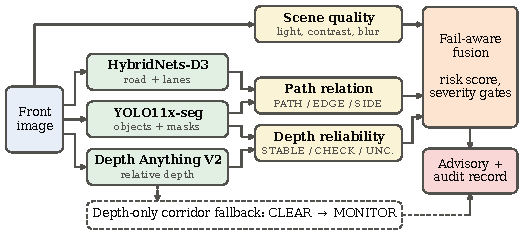
\includegraphics[width=\columnwidth]{figures/fig_pipeline.pdf}
\caption{Fail-aware fusion pipeline. Component outputs remain explicit until reliability and geometry gating; the depth-only fallback can only raise \st{Clear} to \st{Monitor}.}
\label{fig:pipeline}
\end{figure}

\subsection{Complementary Evidence}
The system combines three pretrained perception sources (Fig.~\ref{fig:pipeline}): YOLO11 object classes, confidences, boxes, and instance masks~\cite{ultralytics}; HybridNets drivable-area and lane masks, used to estimate an internal ego corridor~\cite{hybridnets}; and a Depth Anything V2 relative-depth field~\cite{dav2}. No component is trained or fine-tuned for this work. Object evidence comes from the detector only: road and depth cues can change an advisory, but they never create an object or verify a driving action. Depth is used only as a relative cue, never as metric distance, speed, or time-to-collision. Uncertainty is handled asymmetrically: weak evidence lowers the confidences below and can add caution (the fallback turns \st{Clear} into \st{Monitor}), but the gates of Sec.~\ref{sec:advisory} keep it from justifying \st{Brake} or \st{Stop}.

\subsection{Scene and Object-Depth Reliability}
Scene quality is estimated from the gray image: median illumination $m$, the 10--90 percentile range $R$, and the Laplacian variance $v$. With $q_{\mathrm{illum}}=\mathrm{clip}((m-18)/72)$, $q_{\mathrm{contrast}}=\mathrm{clip}((R-20)/80)$, and $q_{\mathrm{sharp}}$ the log-scaled variance between 12 and 500, all clipped to $[0,1]$, \mbox{$q_s = 0.40\,q_{\mathrm{illum}} + 0.30\,q_{\mathrm{contrast}} + 0.30\,q_{\mathrm{sharp}}$}. Low light ($m<45$), low contrast ($R<55$), blur ($v<60$), and glare are kept as separate flags; a scene is \st{Degraded} when $q_s<0.35$ or it is both dark and blurred, and \st{Limited} when $q_s<0.58$ or any flag is raised.

Depth Anything V2 outputs an affine-invariant inverse-depth response $d$ in which larger values are nearer~\cite{dav2,midas}. The pipeline converts it into a relative depth index \mbox{$u=\mathrm{clip}(1000/d,\,0.1,\,999)$}, so that a \emph{smaller} $u$ means a \emph{nearer} surface. Because $d$ has an unknown scale and shift, $u$ preserves only the within-image ordering; it is not a distance and is never compared across images.

For each accepted object, $u$ is sampled in three regions of the eroded instance mask: a center region, a lower-body region, and an inner-core region (Fig.~\ref{fig:regions}). Let $u_r$ be the trimmed (12--88 percentile) median in region $r$ and $n_r$ its number of retained pixels. The object estimate is the support-weighted geometric mean $u_o=\exp(\sum_r w_r\log u_r/\sum_r w_r)$ with $w_r=\min(n_r,300)$, and regional consistency is measured by the disagreement ratio $a=\max_r u_r/\min_r u_r$. With $s$ the 20--80 interquantile spread of all sampled values normalized by $u_o$ and $N$ the number of retained pixels, the base reliability is
\begin{equation}
c_u = \mathrm{clip}(1.35/a,0,1)\, e^{-0.85 s}\, \mathrm{clip}(N/120,\,0.25,\,1),
\label{eq:cu}
\end{equation}
which is then multiplied by a mask-quality factor $\mathrm{clip}(0.45+0.75\,m_q,\,0.35,\,1)$ (where $m_q$ penalizes nearly empty or box-like masks), by $0.58$ when only a box is available, and by $0.72$ or $0.82$ for objects truncated by the side/top or bottom image border. The estimate is \st{Stable} when $c_u \ge 0.68$ and $a \le 1.35$, \st{Check} when $c_u \ge 0.35$ and $a \le 1.80$, and \st{Uncertain} otherwise. The constants were fixed during development, before the evaluation reported here; Section~\ref{sec:sensitivity} reports their sensitivity.

\begin{figure}[t]
\centering
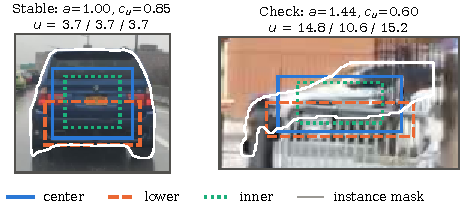
\includegraphics[width=\columnwidth]{figures/fig_regions.pdf}
\caption{Multi-region depth sampling. Left: the three regions of a vehicle agree, so the estimate is \st{Stable}. Right: the mask leaks into the background, the regions disagree, and the estimate is kept at \st{Check}.}
\label{fig:regions}
\end{figure}

\subsection{Path Relation and Conservative Advisory}
\label{sec:advisory}
The ego corridor is a perspective band that starts at 35\% of the image height and widens toward the bottom; its center and width follow the HybridNets lane pixels in the rows where both lane boundaries are visible and keep the default trapezoid elsewhere. An object is \st{Path} when its ground-contact point lies inside the corridor or at least 10\% of the lower 30\% of its mask overlaps it, \st{Edge} when it overlaps a dilated corridor, and \st{Side} otherwise.

A risk score combines the relative depth index, image area, bottom position, path relation ($+32$ for \st{Path}, $+15$ for \st{Edge}), and a vulnerable-road-user bonus, and is mapped to \st{Clear}, \st{Monitor}, \st{Slow}, \st{Brake}, or \st{Stop} at the cut-offs 24, 40, 60, and 78. The evidence confidence combines detector confidence $c_{\mathrm{det}}$, depth reliability $c_u$, a distance-agreement score $c_d$, and scene quality:
\begin{equation}
c_e=\sqrt{c_{\mathrm{det}}\,\max(c_u,c_d)}\;(0.65+0.35\,q_s).
\label{eq:ce}
\end{equation}
Here $c_d$ measures the agreement of up to three monocular distance cues (depth fitted to the road plane, ground-contact geometry, and class-height priors) under default camera assumptions (1.5\,m height, 70$^\circ$ field of view). It is used only as an agreement score inside~\eqref{eq:ce} and the weak-evidence gates; no metric distance is reported.

Severity gates then cap unsupported outputs and can only lower an advisory: (i)~a \st{Side} object raises at most \st{Monitor}, or \st{Slow} for a close vulnerable road user at the image bottom; (ii)~an \st{Edge} object raises at most \st{Brake}; (iii)~\st{Stop} requires a \st{Stable}, very near \st{Path} object ($u_o\le4$ with $c_u\ge0.60$, at least 2.5\% of the image area, and its lower edge in the bottom 32\% of the image, or a distance cue of at most 4\,m with $c_d\ge0.55$) with $c_{\mathrm{det}}\ge0.55$ and $c_e\ge0.48$; (iv)~\st{Brake} requires a credible size or position, $c_{\mathrm{det}}\ge0.30$, and $c_e\ge0.28$; (v)~an \st{Uncertain} object with $c_{\mathrm{det}}<0.35$ raises at most \st{Monitor}; and (vi)~in a degraded scene ($q_s<0.35$), \st{Brake} also requires a \st{Stable} object with $c_{\mathrm{det}}\ge0.45$. A failed gate lowers the advisory by one level.

\subsection{Depth-Only Corridor Fallback and Audit Record}
Detector-empty images should not automatically be treated as safe. The corridor is divided into far, middle, and near bands, and the median $u$ of road pixels in each band is checked for the expected monotonic order. The corridor state is \st{Unavailable} when fewer than 55\% of the band pixels are valid or a band is missing, \st{Limited} when the scene is degraded or the band confidence is below 0.38, \st{Check} when the ordering is violated, and \st{Consistent} otherwise. When no object is accepted and the state is not \st{Consistent}, the global advisory is raised from \st{Clear} to \st{Monitor}. The fallback never creates an object, a location, or a distance.

The output is the global advisory plus one audit record per accepted object (class, confidences, mask source, $u_o$, reliability state, path relation, risk score, and advisory), so every advisory can be traced to its evidence. A \st{Stable} state indicates regional agreement, not ground-truth correctness.

\section{Experimental Protocol}
\subsection{Models and Inference Profile}
YOLO11x-seg (COCO-pretrained) runs at 960\,px with a confidence threshold of 0.15 and four test-time passes (raw and scene-adaptively enhanced input, each with a horizontal flip) fused by weighted box fusion; single-pass detections below 0.34 are rejected. Enhancement (gamma, luma CLAHE, mild unsharp masking) is applied to the YOLO input only, when the scene flags call for it. HybridNets-D3 runs at 640\,px and Depth Anything V2 ViT-L at 518\,px. All thresholds and fusion rules are fixed across every evaluation; the code is commit \texttt{\CodeCommit}, and the weight checksums are listed in the repository.

\subsection{Evaluation Data}
All headline experiments use the 10{,}000 BDD100K validation images~\cite{bdd100k}, whose labels none of the three networks was trained on. A random 500-image \emph{dev} subset (seed \SplitSeed) is used only for threshold sensitivity, the operating curve, and the dataset-average priors of the ablations. The remaining 9{,}500 images form the \emph{test} split on which every headline number is computed (ID-list SHA-256 prefix \texttt{\TestIDsHash}). The \emph{hard} set is a deterministic stress subset of the test split: all validation images are measured at $320\times180$ (mean brightness $b$, standard deviation $c$, Laplacian variance $l$, dark and bright pixel fractions $f_d$ ($\le35$) and $f_b$ ($\ge245$), Canny-edge density $e$), each normalized between its 2nd and 98th percentiles; the category scores are $0.65f_d+0.35(1-b)$ (dark), $1-c$ (low contrast), $1-l$ (blur), $0.75f_b+0.25b$ (glare), and $e$ (complex), and each category in turn keeps its 20 highest-scoring images not already selected (prefix \texttt{\HardIDsHash}). Perturbation stability is also measured on a random 1{,}000-image subset of the test split (the \emph{1k subset})\ifdefined\OpValopImages, and the \OpValopImages{} test images outside the hard set and the 1k subset (\emph{val\_rest}) serve as a held-out check of the operating point chosen on the dev subset\fi.\ifdefined\TrainImages{} As a supplementary check, the same protocol is applied to the \TrainImages{} annotated BDD100K \emph{train} images (labels from public copies that reproduce all 10{,}000 validation labels and masks exactly); HybridNets was trained on them, so they are reported separately.\fi

\subsection{Ground-Truth Protocol}
BDD100K validation annotations provide boxes with occlusion and truncation flags, time-of-day and weather tags, and drivable-area maps that separate the \emph{direct} (ego) lane from \emph{alternative} lanes~\cite{bdd100k}. A \emph{road user} is any annotated person, rider, or vehicle; it is \emph{relevant} when its box is at least 5\% of the image height (36\,px, roughly within 40\,m for a car). Its ground-truth lane is the drivable label under a ground-contact strip just below the box (direct or alternative when those labels cover at least a quarter of the strip). Detections are matched class-agnostically to road users at IoU $\ge 0.5$. An image is \emph{occupied} when a relevant road user stands in the direct lane. An \emph{unsafe \st{Clear}} is a \st{Clear} advisory on an occupied image; \emph{over-caution} is \st{Slow} or higher when no road user of any size is in the direct lane (an upper bound: an adjacent-lane hazard can justify such advisories); and a \st{Brake}/\st{Stop} advisory is \emph{unsupported} when none of the objects that raised it is a true positive in the direct or alternative lane. These definitions were fixed before any result was inspected.

\subsection{Ablations, Replays, and Statistics}
Each ablation re-runs only the fusion stage on identical network outputs, so all comparisons are paired; replaying the published constants reproduces the original reports byte for byte. The cumulative baselines are B0, YOLO with dataset-average road and depth priors from the dev subset; B1, which adds the HybridNets corridor; B2, which adds Depth Anything V2 sampled in the center region only; and B3, which adds the multi-region reliability and scene quality. The full system adds the severity gates and the fallback. Stability is measured under six mild perturbations (darker and brighter gamma, 0.7 contrast, Gaussian blur with $\sigma=1.5$, Gaussian noise with $\sigma=8$, and JPEG quality 35). Proportions use Wilson intervals~\cite{wilson1927}; object-level ratios use an image-level cluster bootstrap with 10{,}000 resamples~\cite{efron1993}, because detections in one image are not independent; and paired image-level outcomes use the exact McNemar test~\cite{mcnemar1947}.\ifdefined\TestTFourImages{} Inference for \TestTFourImages{} test images and every perturbation run of the 1k subset ran on an NVIDIA T4 with the same pinned library versions; perturbed images are always compared with clean runs from the same GPU.\fi

\section{Results}
\begin{table}[t]
\centering
\caption{Internal reliability and ground-truth results}
\label{tab:overall}
\footnotesize
\setlength{\tabcolsep}{3pt}
\begin{tabular}{lcc}
\hline
Measure & Hard (100) & Test (9{,}500) \\
\hline
Accepted detections & 505 & 75{,}819 \\
\textsc{Stable}/\textsc{Check}/\textsc{Uncertain} & 437/67/1 & 64{,}334/11{,}104/354 \\
Stable ratio, Wilson 95\% CI & 86.5 [83.3, 89.2] & 84.9 [84.6, 85.1] \\
Stable ratio, image-bootstrap CI & 86.5 [83.5, 89.2] & 84.9 [84.6, 85.1] \\
\hline
Detection precision (GT) & 86.3 [82.9, 89.6] & 89.1 [88.8, 89.4] \\
Recall, relevant road users & 72.2 [67.2, 77.3] & 78.9 [78.4, 79.3] \\
\textsc{Path} precision (matched) & 15.8 [11.0, 22.3] & 9.2 [8.8, 9.5] \\
\textsc{Path} recall (matched) & 56.8 [42.2, 70.3] & 53.8 [52.3, 55.2] \\
Corridor IoU with GT ego lane & 0.242 & 0.240 \\
\hline
Occupied images & 30 & 3{,}250 \\
Unsafe \textsc{Clear}, fallback on & 0/30 (0.0) & 11/3{,}250 (0.3) \\
Unsafe \textsc{Clear}, fallback off & 1/30 (3.3) & 15/3{,}250 (0.5) \\
Over-caution (free ego lane) & 34/67 (50.7) & 4{,}799/5{,}844 (82.1) \\
Unsupported \textsc{Brake}/\textsc{Stop} & 31/47 & 4{,}179/6{,}188 \\
Detector-empty / fallback fired & 15/15 & 295/236 \\
\hline
\end{tabular}
\end{table}


\subsection{Internal Reliability and Detection Correctness}
Table~\ref{tab:overall} summarizes the test split and the hard set. On the test split, \TestStable{} of \TestAccepted{} accepted detections are \st{Stable} (\TestStablePct\%, image-bootstrap CI \TestStableBootLow--\TestStableBootHigh\%); on the hard set the ratio is \HardStablePct\% (Wilson CI \HardStableLow--\HardStableHigh\%), close to the 86.1\% of the submitted version.\footnote{The submitted version reported 596 detections on a hard set whose image list was not preserved; every number here comes from the regenerated, published splits.} Against the annotations, the accepted test detections reach \TestPrec\% precision and \TestRecRel\% recall of relevant road users; relative to the raw YOLO ensemble (\TestRawPrec\% precision, \TestRawRecRel\% recall), the fusion-level suppression trades a little recall for precision.

\begin{table}[t]
\centering
\caption{Reliability states against BDD100K annotations (test set, \%)}
\label{tab:states_test}
\footnotesize
\setlength{\tabcolsep}{3pt}
\begin{tabular}{lccccc}
\hline
State & $n$ & False positive & Occl. & Trunc. & IoU \\
\hline
\textsc{Stable} & 64{,}334 & 9.7 [9.5, 10.0] & 59.0 & 2.5 & 0.825 \\
\textsc{Check} & 11{,}104 & 16.5 [15.8, 17.2] & 35.5 & 69.2 & 0.849 \\
\textsc{Uncertain} & 354 & 44.1 [38.9, 49.3] & 54.5 & 7.1 & 0.716 \\
\hline
\end{tabular}
\end{table}


\subsection{Do Reliability States Mean Anything?}
Table~\ref{tab:states_test} relates the reliability states to the annotations. Non-\st{Stable} test estimates are false positives in \TestFPNonStable\% of cases (CI \TestFPNonStableLow--\TestFPNonStableHigh\%) against \TestFPStable\% for \st{Stable} ones (CI \TestFPStableLow--\TestFPStableHigh\%), a factor of \TestFPRatio. \st{Check} concentrates on objects truncated by the image border (\TestTruncCheck\% vs.\ \TestTruncStable\%), exactly the case where regional depth samples cannot agree. The states are thus informative about correctness, although \st{Stable} remains an agreement measure, not a depth-accuracy guarantee.

\subsection{Advisories, Path Relation, and the Cost of Conservatism}
Unsafe \st{Clear} occurs on \TestUnsafe{} of \TestOccupied{} occupied test images (Wilson upper bound \TestUnsafeHigh\%) and on \HardUnsafe{} of \HardOccupied{} occupied hard-set images.\ifdefined\TestUnsafeDetected{} In \TestUnsafeDetected{} of the \TestUnsafe{} test cases the in-lane road user was detected, but the corridor classified it as \st{Side}, which caps its advisory; in the other \TestUnsafeMissed{} the detector missed it (\TestUnsafeMissedNight{} at night)\ifdefined\TrainUnsafeDetected{}; the \TrainUnsafe{} train cases split the same way (\TrainUnsafeDetected{} and \TrainUnsafeMissed{})\fi.\fi{} This has a cost: only \TestClearPct\% of test images receive \st{Clear} and \TestSeverePct\% receive \st{Brake} or \st{Stop}, over-caution affects \TestOver{} of \TestFree{} free-lane images, and \TestUnsupportedPct\% of \st{Brake}/\st{Stop} advisories are unsupported by an in-lane object. The main cause is the ego corridor. Matched \st{Path} precision is only \TestPathPrec\% (recall \TestPathRec\%) because the perspective band is wider than the true ego lane near the vanishing point, so roadside and distant road users are labeled \st{Path} (\TestPathOff{} of the \TestPathPrecN{} matched \st{Path} objects stand outside the annotated drivable area). The corridor overlaps the annotated ego lane with IoU \TestCorridorIoU, although the HybridNets road mask itself matches the annotated drivable area with IoU \TestRoadIoU. Part of the disagreement is annotation: on unmarked streets the BDD100K direct lane often spans the whole carriageway. Fig.~\ref{fig:qualitative} shows both behaviors, and Fig.~\ref{fig:operating} places the published cut-offs on the trade-off between unsafe \st{Clear} and over-caution. On the dev subset, the cut-offs can be relaxed up to $\times$\OpDevSafeScale{} before the first unsafe \st{Clear}, which lowers over-caution from \OpDevBaseOverPct\% to \OpDevSafeOverPct\%\ifextended{} (at $\times$\OpDevMaxScale{} it falls to \OpDevMaxOverPct\% while \OpDevMaxUnsafePct\% of occupied images receive \st{Clear})\fi; \ifdefined\OpValopChosenUnsafe on the \OpValopImages{} held-out val\_rest images the same relaxation raises unsafe \st{Clear} from \OpValopBaseUnsafe{} to \OpValopChosenUnsafe{} of \OpValopOccupied{} occupied images (\OpValopBaseUnsafePct\% to \OpValopChosenUnsafePct\%, upper bound \OpValopChosenUnsafeHigh\%) while over-caution falls from \OpValopBaseOverPct\% to \OpValopChosenOverPct\%\ifextended\ifdefined\OpTrainChosenUnsafe{}, and on the \OpTrainImages{} train images unsafe \st{Clear} moves from \OpTrainBaseUnsafePct\% to \OpTrainChosenUnsafePct\% and over-caution from \OpTrainBaseOverPct\% to \OpTrainChosenOverPct\%\fi\fi. A margin chosen on the \DevImages{} dev images therefore does not transfer, and the published cut-offs are kept.\else on the 1k test subset the same relaxation changes unsafe \st{Clear} from \OpStdBaseUnsafe{} to \OpStdAtSafeUnsafe{} of \OpStdOccupied{} occupied images.\fi

\begin{figure*}[t]
\centering
\ifextended
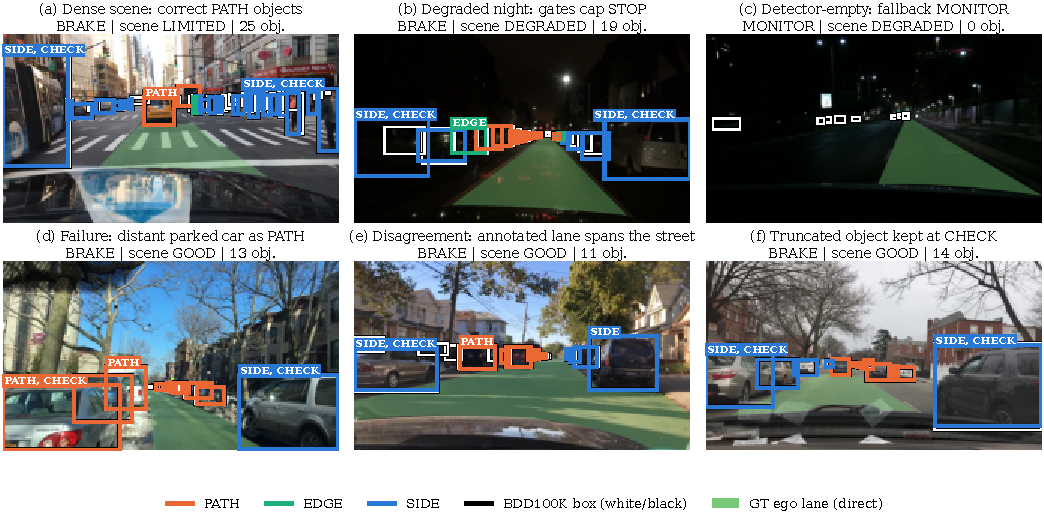
\includegraphics[width=\textwidth]{figures/fig_qualitative.pdf}
\caption{Hard-set cases selected by fixed rules: three intended behaviors (a--c) and three failure modes or annotation disagreements (d--f). Colored boxes are system outputs labeled by path relation (\st{Check} marks a depth estimate that is not \st{Stable}; small boxes are unlabeled); white boxes are BDD100K annotations; the green tint is the annotated ego lane.}
\else
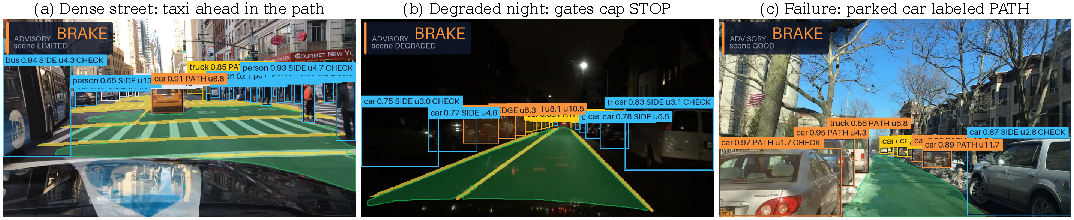
\includegraphics[width=\textwidth]{figures/fig_qualitative_main.pdf}
\caption{Hard-set cases selected by fixed rules, drawn with the system's overlay: (a)~the taxi and truck ahead are \st{Path} and raise \st{Brake}; (b)~in a degraded night scene the gates cap \st{Stop} at \st{Brake}; (c)~failure: cars parked at the curb fall inside the corridor and are labeled \st{Path}. Every box is labeled with class, detector confidence, path relation, and relative depth index~$u$, followed by \st{Check} when the depth is not \st{Stable}; box and label color: advisory of that object (blue \st{Monitor}, yellow \st{Slow}, orange \st{Brake}); green: HybridNets road, yellow: lanes.}
\fi
\label{fig:qualitative}
\end{figure*}

\begin{figure}[t]
\centering
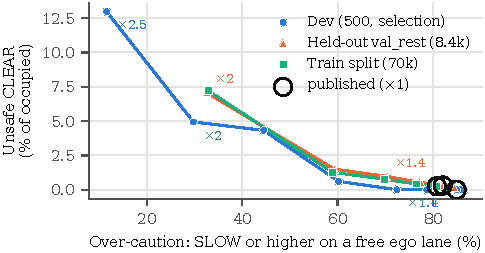
\includegraphics[width=\columnwidth]{figures/fig_operating.pdf}
\caption{Operating curve: all advisory cut-offs scaled together (dev subset: $\times0.5$ to $\times2.5$\ifdefined\OpValopImages; held-out val\_rest\ifdefined\OpTrainImages{} and train split\fi: $\times0.8$ to $\times2.0$\fi; circled points: published constants).}
\label{fig:operating}
\end{figure}

\begin{table}[t]
\centering
\caption{Cumulative build-up on the test set (\%). Flip: advisory change under mild perturbation (hard set)}
\label{tab:buildup_test}
\footnotesize
\setlength{\tabcolsep}{3pt}
\begin{tabular}{lccccc}
\hline
Configuration & Unsafe & \% & Over-c. & Severe & Flip \\
\hline
B0: YOLO only (road/depth priors) & 17/3{,}250 & 0.5 & 86.7 & 66.8 & 13.0 \\
B1: + HybridNets corridor & 16/3{,}250 & 0.5 & 88.4 & 65.3 & -- \\
B2: + DA V2, single region & 15/3{,}250 & 0.5 & 88.1 & 74.3 & -- \\
B3: + multi-region, scene quality & 15/3{,}250 & 0.5 & 88.2 & 74.5 & 14.5 \\
Full: + gates, fallback (proposed) & 11/3{,}250 & 0.3 & 82.1 & 65.1 & 8.3 \\
\hline
\end{tabular}
\end{table}


\subsection{Ablations}
\label{sec:ablations}
Table~\ref{tab:buildup_test} builds the system up from YOLO alone on the test split, and leave-one-out replays isolate each component on identical network outputs. Against the YOLO-only baseline B0, the full system is less over-cautious (\TestOverPct\% vs.\ \TestBZeroOverPct\%, $p\TestBZeroOverP$) with no more unsafe \st{Clear} (\TestUnsafe{} vs.\ \TestBZeroUnsafe). The severity gates mainly control the aggressive outputs: removing them changes \st{Stop} advisories from \TestStop{} to \TestNoGatesStop{}, over-caution from \TestOver{} to \TestNoGatesOver{} images (McNemar $p\TestNoGatesOverP$), and unsupported \st{Brake}/\st{Stop} outputs from \TestUnsupported{} to \TestNoGatesUnsupported. The fallback fired on \TestFallback{} of the \TestEmpty{} detector-empty test images; without it, unsafe \st{Clear} changes from \TestUnsafe{} to \TestUnsafeNoFB{} ($p\TestNoFBUnsafeP$). Scene quality feeds the same mechanism: without it, the depth-only scan of degraded detector-empty images looks consistent, and \st{Clear} images change from \TestClear{} to \TestNoSQClear. Multi-region sampling mainly changes the reliability states (stable ratio \TestSingleStablePct\% with the center region alone vs.\ \TestStablePct\%) rather than the advisories (\TestSingleChanged{} changed images).

The two dense sources contribute very differently. Replacing Depth Anything V2 with a dataset-average depth prior changes \TestNoDepthChanged{} test advisories and the stable ratio to \TestNoDepthStablePct\%, so per-image depth drives both the reliability states and the severity. Replacing HybridNets with an average road prior changes only \TestNoHybChanged{} advisories, because the corridor follows the lanes only where both boundaries are visible: on average only \TestLaneGuidedPct\% of corridor rows are lane-guided, and \TestMostlyTrapezoidPct\% of test images use the default trapezoid for more than three quarters of the corridor. HybridNets is therefore under-used rather than unreliable (Section~\ref{sec:discussion}).

\ifextended\begin{table}[t]
\centering
\caption{Results by difficulty category, time of day, and weather (\%)}
\label{tab:groups}
\footnotesize
\setlength{\tabcolsep}{3pt}
\begin{tabular}{lcccccc}
\hline
Group & Img. & Obj. & Stable & Prec. & Rec. & Unsafe \textsc{Clear} \\
\hline
\multicolumn{7}{l}{\emph{Hard set, by difficulty category}} \\
Blur & 20 & 43 & 81.4 & 83.7 & 56.9 & 0/3 \\
Dark & 20 & 52 & 90.4 & 82.7 & 66.1 & 0/2 \\
Low contrast & 20 & 93 & 81.7 & 72.0 & 69.0 & 0/7 \\
Glare & 20 & 110 & 89.1 & 93.6 & 78.4 & 0/5 \\
Complex & 20 & 207 & 87.4 & 90.3 & 77.2 & 0/13 \\
\hline
\multicolumn{7}{l}{\emph{Test split, by time of day and weather}} \\
Daytime & 4{,}993 & 46{,}431 & 86.6 & 92.9 & 83.3 & 7/1{,}944 \\
Dawn/dusk & 739 & 6{,}381 & 85.4 & 91.7 & 82.2 & 0/269 \\
Night & 3{,}734 & 22{,}872 & 81.1 & 80.7 & 70.4 & 4/1{,}027 \\
Clear & 5{,}056 & 36{,}396 & 83.8 & 86.3 & 76.3 & 6/1{,}563 \\
Rainy & 708 & 5{,}155 & 83.3 & 88.5 & 75.9 & 0/220 \\
Snowy & 737 & 5{,}896 & 84.1 & 89.5 & 78.6 & 2/269 \\
Foggy & 13 & 85 & 74.1 & 83.5 & 76.1 & 0/4 \\
\hline
\end{tabular}
\end{table}
\else\begin{table}[t]
\centering
\caption{Test split by time of day and weather (\%)}
\label{tab:groups}
\footnotesize
\setlength{\tabcolsep}{3pt}
\begin{tabular}{lcccccc}
\hline
Group & Img. & Obj. & Stable & Prec. & Rec. & Unsafe \textsc{Clear} \\
\hline
Daytime & 4{,}993 & 46{,}431 & 86.6 & 92.9 & 83.3 & 7/1{,}944 \\
Dawn/dusk & 739 & 6{,}381 & 85.4 & 91.7 & 82.2 & 0/269 \\
Night & 3{,}734 & 22{,}872 & 81.1 & 80.7 & 70.4 & 4/1{,}027 \\
Clear & 5{,}056 & 36{,}396 & 83.8 & 86.3 & 76.3 & 6/1{,}563 \\
Rainy & 708 & 5{,}155 & 83.3 & 88.5 & 75.9 & 0/220 \\
Snowy & 737 & 5{,}896 & 84.1 & 89.5 & 78.6 & 2/269 \\
Foggy & 13 & 85 & 74.1 & 83.5 & 76.1 & 0/4 \\
\hline
\end{tabular}
\end{table}
\fi

\subsection{Difficult Conditions}
Table~\ref{tab:groups} reports \ifextended the hard-set categories and \fi the test split by time of day and weather. Relevant recall is \TestNightRecRel\% at night against \TestDayRecRel\% in daytime, while the stable ratio changes less (\TestNightStablePct\% vs.\ \TestDayStablePct\%): local object-depth agreement can survive darkness, whereas detector recall and scene quality do not. HybridNets remains a reliable road source at night (road IoU \TestNightRoadIoU{} vs.\ \TestDayRoadIoU{}). On the night images, replacing Depth Anything V2 changes \TestNoDepthNightChangedPct\% of the advisories (\TestNoDepthDayChangedPct\% by day) and replacing HybridNets \TestNoHybNightChangedPct\% (\TestNoHybDayChangedPct\%): depth matters equally in both conditions, the road cues about twice as much at night but still far less than depth. Weather is confounded with time of day (\TestWClearNightPct\% of the clear-weather test images are night images, against \TestWRainyNightPct\% of the rainy ones), so it is compared within each time of day: rain lowers relevant recall from \TestWClearDayRecRel\% to \TestWRainyDayRecRel\% by day and from \TestWClearNightRecRel\% to \TestWRainyNightRecRel\% at night (\TestWRainyImages{} rainy images), whereas snow hardly changes it (\TestWSnowyDayRecRel\% and \TestWSnowyNightRecRel\%; \TestWSnowyImages{} images). Fog is too rare in BDD100K (\TestWFoggyImages{} test images) to support any conclusion.\ifdefined\TrainWRainyNightRecRel{} The train split repeats this pattern on \TrainWRainyImages{} rainy and \TrainWSnowyImages{} snowy images (rain: \TrainWClearDayRecRel\% to \TrainWRainyDayRecRel\% by day, \TrainWClearNightRecRel\% to \TrainWRainyNightRecRel\% at night; snow: \TrainWSnowyDayRecRel\% and \TrainWSnowyNightRecRel\%), and fog remains too rare there (\TrainWFoggyImages{} images).\fi\ifextended\ifdefined\TrainNoHybUnsafe{} On the train images, on which HybridNets was trained (road IoU \TrainRoadIoU{} against \TestRoadIoU), unsafe \st{Clear} occurs on \TrainUnsafe{} of \TrainOccupied{} occupied images and over-caution on \TrainOverPct\% of free-lane images (\TrainNoHybUnsafe{} and \TrainNoHybOverPct\% with HybridNets replaced by the dev road prior).\fi\fi

\subsection{Sensitivity, Stability, and Runtime}
\label{sec:sensitivity}
Changing each reliability constant by $\pm20\%$ on the dev subset mainly moves the stable ratio itself (by up to \SensRelStableDelta{} points, almost entirely through the \st{Stable} threshold), whereas the advisories move much less: the \st{Brake}/\st{Stop} rate changes by at most \SensRelSevereDelta{} points (when the \st{Stable} threshold is raised) and over-caution does not change. The advisory trade-off is governed by the risk cut-offs, which is why Fig.~\ref{fig:operating} sweeps them; no sensitivity setting produces an unsafe \st{Clear} on any of the \DevOccupied{} occupied dev images. Under the six mild perturbations, the advisory changes in \StdFlipFull\% of image pairs on the 1k subset and \FlipFull\% on the hard set, against \StdFlipNoGates\% and \FlipNoGates\% without gates; reliability states of persisting objects change in \StdStateFlipFull\% of cases. With the center region alone the flips are essentially unchanged (\StdFlipSingle\% and \FlipSingle\%) and the state changes rise slightly (\StdStateFlipSingle\%): the multi-region check stabilizes the states, not the advisories.\ifdefined\CrossHWFlipFull{} Hardware matters far less: rerunning the clean 1k subset on the T4 instead of the RTX~3050 changes none of its \CrossHWFlipPairsFull{} advisories\ifdefined\CrossHWValFlips{} and \CrossHWValFlips{} of the \CrossHWValPairs{} val\_rest advisories computed on both GPUs\fi.\fi{} On an RTX~3050 laptop GPU the median latency is \LatTotal\,s per image (HybridNets \LatHyb\,s, Depth Anything V2 \LatDepth\,s, four-pass YOLO11x \LatYolo\,s; peak memory \LatVRAM\,GB)\ifdefined\LatTFourTotal{} and \LatTFourTotal\,s on an NVIDIA T4 (\LatTFourImages{} images)\fi, so this configuration is an offline analysis tool, not a real-time module.

\section{Discussion and Limitations}
\label{sec:discussion}
The ground truth supports the fail-aware design where it matters for safety, and shows that the published operating point is conservative in the expensive direction, because a fixed perspective corridor over-assigns roadside and distant objects to the ego path\ifdefined\TestUnsafeDetected{} and, in about half of the unsafe \st{Clear} cases, places a detected in-lane object beside it\fi. The ablations point to a remedy: HybridNets segments the drivable area well, but the corridor rarely uses it. In an exploratory replay that is \emph{not} part of the evaluated method, intersecting the corridor with the dilated HybridNets drivable mask changes matched \st{Path} precision from \TestPathPrec\% to \TestExpPathPrec\% and recall from \TestPathRec\% to \TestExpPathRec\%, and over-caution from \TestOver{} to \TestExpOver{} images, with \TestExpUnsafe{} unsafe \st{Clear}. A corridor that follows the drivable area therefore trades some path recall for less over-caution.

The study has further limitations. Static images cannot show ego speed, object velocity, time-to-collision, or temporal consistency. The ground-truth lane relation is approximated from drivable-area maps, the relevance threshold is a size proxy for distance, and severe weather is under-represented. Depth Anything was trained with unlabeled image collections that include BDD100K imagery~\cite{dav1}, so the depth branch may be favored on this dataset. The four-pass configuration is far from real time. Future work should use the drivable mask in the corridor, calibrated distance targets, video-based temporal evaluation, and human rating of the advisories.

\section{Conclusion}
This paper presented a fail-aware fusion layer for conservative road-hazard assessment from a single front-facing image, which combines YOLO11, HybridNets, and Depth Anything V2 evidence while preserving uncertainty through scene quality, multi-region depth reliability, path reasoning, severity gates, and a depth-only fallback. On 9{,}500 BDD100K validation images and a reproducible hard set, the reliability states align with annotated false positives and truncation, and unsafe \st{Clear} advisories are rare (\TestUnsafe{} of \TestOccupied{} occupied images); the measured price is frequent over-caution caused by an over-inclusive ego corridor. The released code, image-ID manifests, and cached-replay protocol allow every number to be regenerated: \RepoURL.

\ifextended
\appendix
\section*{Supplementary Results}
\begin{table}[t]
\centering
\caption{Leave-one-out ablations on the test set ($p$: exact McNemar test on unsafe \textsc{Clear} vs.\ full)}
\label{tab:loo_test}
\footnotesize
\setlength{\tabcolsep}{3pt}
\begin{tabular}{lccccc}
\hline
Variant & Unsafe & Over-c. & Severe & Changed & $p$ \\
\hline
Full system & 11/3{,}250 & 82.1 & 65.1 & -- & -- \\
w/o HybridNets (road prior) & 13/3{,}250 & 80.3 & 65.6 & 364 & 0.62 \\
w/o DA V2 (depth prior) & 12/3{,}250 & 83.0 & 55.8 & 3{,}631 & 1.00 \\
w/o multi-region (center) & 11/3{,}250 & 82.0 & 65.0 & 47 & 1.00 \\
w/o scene quality in fusion & 14/3{,}250 & 82.4 & 65.7 & 232 & 0.25 \\
w/o severity gates & 11/3{,}250 & 88.2 & 74.5 & 4{,}024 & 1.00 \\
w/o depth-only fallback & 15/3{,}250 & 82.1 & 65.1 & 236 & 0.12 \\
\hline
\end{tabular}
\end{table}

\IfFileExists{tables/train_check.tex}{\begin{table*}[t]
\centering
\caption{Supplementary check on the BDD100K train split. HybridNets was trained on these images, so its road and lane output (and the full-system path measures) are optimistic there; no-HN replaces HybridNets by the dev road prior and is free of that overlap. Rates with Wilson 95\% CIs.}
\label{tab:train}
\footnotesize
\setlength{\tabcolsep}{3pt}
\begin{tabular}{lcccc}
\hline
Measure & Test full (9{,}500) & Test no-HN (9{,}500) & Train full (69{,}863) & Train no-HN (69{,}863) \\
\hline
Detection precision (GT) & 89.1 & 91.3 & 88.9 & 91.2 \\
Recall, relevant road users & 78.9 & 76.0 & 79.4 & 76.6 \\
\textsc{Path} precision & 9.2 & 9.9 & 9.1 & 9.8 \\
\textsc{Path} recall & 53.8 & 54.4 & 53.3 & 54.0 \\
Road IoU (HybridNets vs GT) & 0.828 & -- & 0.854 & -- \\
Ego-corridor IoU & 0.240 & -- & 0.237 & -- \\
\hline
Unsafe \textsc{Clear} (\% occupied) & 0.34 [0.19, 0.61] & 0.40 [0.23, 0.68] & 0.26 [0.20, 0.33] & 0.40 [0.33, 0.49] \\
Over-caution (\% free lane) & 82.1 [81.1, 83.1] & 80.3 [79.3, 81.3] & 80.8 [80.4, 81.2] & 79.1 [78.7, 79.5] \\
\textsc{Brake}/\textsc{Stop} (\% images) & 65.1 & 65.6 & 64.9 & 65.4 \\
\hline
\end{tabular}
\end{table*}
}{}
\begin{table}[t]
\centering
\caption{Advisory stability under six mild photometric perturbations (\%): advisory flips, severe flips, and reliability-state flips of persisting objects}
\label{tab:stability}
\footnotesize
\setlength{\tabcolsep}{3pt}
\begin{tabular}{lccccc}
\hline
Variant & Hard flip & Hard sev. & 1k flip & 1k sev. & State \\
\hline
Full system & 8.3 & 3.7 & 5.2 & 2.0 & 3.0 \\
w/o severity gates & 12.2 & 6.2 & 6.6 & 2.8 & 3.0 \\
w/o multi-region & 8.7 & 3.8 & 5.1 & 2.0 & 3.4 \\
w/o scene quality & 11.2 & 4.5 & 5.2 & 2.4 & 3.0 \\
B3 (no gates, no fallback) & 14.5 & 8.0 & 6.5 & 3.0 & 3.0 \\
B0 (YOLO only) & 13.0 & 8.5 & 6.8 & 3.2 & 3.9 \\
\hline
\end{tabular}
\end{table}

\begin{table}[t]
\centering
\caption{Threshold sensitivity on the dev split (\%)}
\label{tab:sensitivity}
\footnotesize
\setlength{\tabcolsep}{3pt}
\begin{tabular}{lcccc}
\hline
Setting (dev set) & Stable & Unsafe & Over-c. & Severe \\
\hline
Published constants & 85.1 & 0/162 & 85.0 & 65.8 \\
stable\_c=0.544 & 96.4 & 0/162 & 85.0 & 65.8 \\
stable\_c=0.816 & 51.2 & 0/162 & 85.0 & 60.8 \\
stable\_a=1.08 & 80.7 & 0/162 & 85.0 & 65.4 \\
stable\_a=1.62 & 85.2 & 0/162 & 85.0 & 65.8 \\
check\_c=0.28 & 85.1 & 0/162 & 85.0 & 65.8 \\
check\_c=0.42 & 85.2 & 0/162 & 85.0 & 65.8 \\
check\_a=1.44 & 85.2 & 0/162 & 85.0 & 65.8 \\
check\_a=2.16 & 85.1 & 0/162 & 85.0 & 65.8 \\
k\_ratio=1.08 & 84.3 & 0/162 & 85.0 & 65.8 \\
k\_ratio=1.62 & 85.1 & 0/162 & 85.0 & 65.8 \\
k\_spread=0.68 & 86.2 & 0/162 & 85.0 & 65.8 \\
k\_spread=1.02 & 83.9 & 0/162 & 85.0 & 65.8 \\
n\_support=96 & 85.4 & 0/162 & 85.0 & 65.8 \\
n\_support=144 & 84.5 & 0/162 & 85.0 & 65.8 \\
risk scale=0.8 & 85.1 & 0/162 & 85.9 & 68.4 \\
risk scale=0.9 & 85.1 & 0/162 & 85.9 & 67.4 \\
risk scale=1.1 & 85.1 & 0/162 & 83.1 & 61.2 \\
risk scale=1.2 & 85.1 & 0/162 & 78.7 & 50.8 \\
SQ w=0.3333,0.3333,0.3334 & 85.1 & 0/162 & 85.0 & 65.8 \\
SQ w=0.5,0.25,0.25 & 85.1 & 0/162 & 85.0 & 65.6 \\
SQ w=0.2,0.4,0.4 & 85.1 & 0/162 & 85.0 & 65.8 \\
\hline
\end{tabular}
\end{table}

\begin{table}[t]
\centering
\caption{Cumulative build-up on the hard set (\%). Flip: advisory change under mild perturbation (hard set)}
\label{tab:buildup_hard}
\footnotesize
\setlength{\tabcolsep}{3pt}
\begin{tabular}{lccccc}
\hline
Configuration & Unsafe & \% & Over-c. & Severe & Flip \\
\hline
B0: YOLO only (road/depth priors) & 1/30 & 3.3 & 59.7 & 49.0 & 13.0 \\
B1: + HybridNets corridor & 1/30 & 3.3 & 62.7 & 47.0 & -- \\
B2: + DA V2, single region & 1/30 & 3.3 & 59.7 & 54.0 & -- \\
B3: + multi-region, scene quality & 1/30 & 3.3 & 61.2 & 55.0 & 14.5 \\
Full: + gates, fallback (proposed) & 0/30 & 0.0 & 50.7 & 47.0 & 8.3 \\
\hline
\end{tabular}
\end{table}

\begin{table}[t]
\centering
\caption{Reliability states against BDD100K annotations (hard set, \%)}
\label{tab:states_hard}
\footnotesize
\setlength{\tabcolsep}{3pt}
\begin{tabular}{lccccc}
\hline
State & $n$ & False positive & Occl. & Trunc. & IoU \\
\hline
\textsc{Stable} & 437 & 11.9 [8.9, 15.1] & 58.7 & 2.1 & 0.807 \\
\textsc{Check} & 67 & 23.9 [13.9, 34.2] & 33.3 & 78.4 & 0.863 \\
\textsc{Uncertain} & 1 & 100.0 [100.0, 100.0] & -- & -- & -- \\
\hline
\end{tabular}
\end{table}

\begin{figure}[t]
\centering
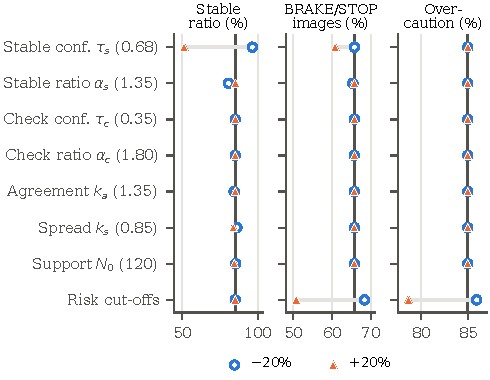
\includegraphics[width=\columnwidth]{figures/fig_sensitivity.pdf}
\caption{Sensitivity on the dev subset: each fusion constant is changed by $\pm20\%$ (the risk cut-offs are scaled together). Vertical rules mark the published constants.}
\label{fig:sensitivity}
\end{figure}
\fi

% Balances the two columns of the last page (main version only); adjust the number if the text length changes.
\begin{thebibliography}{99}
\bibitem{bdd100k} F. Yu \emph{et al.}, ``BDD100K: A diverse driving dataset for heterogeneous multitask learning,'' in \emph{Proc. IEEE/CVF Conf. Computer Vision and Pattern Recognition (CVPR)}, 2020, pp. 2636--2645.
\bibitem{dav2} L. Yang, B. Kang, Z. Huang, Z. Zhao, X. Xu, J. Feng, and H. Zhao, ``Depth Anything V2,'' arXiv preprint arXiv:2406.09414, 2024.
\bibitem{geifman2017} Y. Geifman and R. El-Yaniv, ``Selective classification for deep neural networks,'' in \emph{Proc. Advances in Neural Information Processing Systems (NeurIPS)}, 2017.
\bibitem{rahman2021} Q. M. Rahman, P. Corke, and N. S\"underhauf, ``Run-time monitoring of machine learning for robotic perception: A survey of emerging trends,'' \emph{IEEE Access}, vol. 9, pp. 20067--20075, 2021.
\bibitem{hybridnets} D. Vu, B. Ngo, and H. Phan, ``HybridNets: End-to-end perception network,'' arXiv preprint arXiv:2203.09035, 2022.
\bibitem{ultralytics} Ultralytics, ``Ultralytics YOLO documentation.'' [Online]. Available: https://docs.ultralytics.com/. Accessed: Jun. 13, 2026.
\bibitem{yolo} J. Redmon, S. Divvala, R. Girshick, and A. Farhadi, ``You only look once: Unified, real-time object detection,'' in \emph{Proc. IEEE Conf. Computer Vision and Pattern Recognition (CVPR)}, 2016, pp. 779--788.
\bibitem{yolop} D. Wu, M.-W. Liao, W.-T. Zhang, X.-G. Wang, X. Bai, W.-Q. Cheng, and W.-Y. Liu, ``YOLOP: You only look once for panoptic driving perception,'' \emph{Machine Intelligence Research}, vol. 19, no. 6, pp. 550--562, 2022.
\bibitem{midas} R. Ranftl, K. Lasinger, D. Hafner, K. Schindler, and V. Koltun, ``Towards robust monocular depth estimation: Mixing datasets for zero-shot cross-dataset transfer,'' \emph{IEEE Trans. Pattern Analysis and Machine Intelligence}, vol. 44, no. 3, pp. 1623--1637, 2022.
\bibitem{dav1} L. Yang, B. Kang, Z. Huang, X. Xu, J. Feng, and H. Zhao, ``Depth Anything: Unleashing the power of large-scale unlabeled data,'' in \emph{Proc. IEEE/CVF Conf. Computer Vision and Pattern Recognition (CVPR)}, 2024.
\bibitem{guo2017} C. Guo, G. Pleiss, Y. Sun, and K. Q. Weinberger, ``On calibration of modern neural networks,'' in \emph{Proc. 34th Int. Conf. Machine Learning (ICML)}, 2017, pp. 1321--1330.
\bibitem{kendall2017} A. Kendall and Y. Gal, ``What uncertainties do we need in Bayesian deep learning for computer vision?'' in \emph{Proc. Advances in Neural Information Processing Systems (NeurIPS)}, 2017.
\bibitem{ensembles} B. Lakshminarayanan, A. Pritzel, and C. Blundell, ``Simple and scalable predictive uncertainty estimation using deep ensembles,'' in \emph{Proc. Advances in Neural Information Processing Systems (NeurIPS)}, 2017.
\bibitem{poggi2020} M. Poggi, F. Aleotti, F. Tosi, and S. Mattoccia, ``On the uncertainty of self-supervised monocular depth estimation,'' in \emph{Proc. IEEE/CVF Conf. Computer Vision and Pattern Recognition (CVPR)}, 2020.
\bibitem{hornauer2022} J. Hornauer and V. Belagiannis, ``Gradient-based uncertainty for monocular depth estimation,'' arXiv preprint arXiv:2208.02005, 2022.
\bibitem{conformal} A. N. Angelopoulos and S. Bates, ``A gentle introduction to conformal prediction and distribution-free uncertainty quantification,'' arXiv preprint arXiv:2107.07511, 2021.
\bibitem{feng2020} D. Feng, A. Harakeh, S. L. Waslander, and K. Dietmayer, ``A review and comparative study on probabilistic object detection in autonomous driving,'' arXiv preprint arXiv:2011.10671, 2020.
\bibitem{bijelic2020} M. Bijelic, T. Gruber, F. Mannan, F. Kraus, W. Ritter, K. Dietmayer, and F. Heide, ``Seeing through fog without seeing fog: Deep multimodal sensor fusion in unseen adverse weather,'' in \emph{Proc. IEEE/CVF Conf. Computer Vision and Pattern Recognition (CVPR)}, 2020.
\bibitem{wilson1927} E. B. Wilson, ``Probable inference, the law of succession, and statistical inference,'' \emph{J. American Statistical Association}, vol. 22, no. 158, pp. 209--212, 1927.
\bibitem{efron1993} B. Efron and R. J. Tibshirani, \emph{An Introduction to the Bootstrap}. New York, NY, USA: Chapman \& Hall, 1993.
\bibitem{mcnemar1947} Q. McNemar, ``Note on the sampling error of the difference between correlated proportions or percentages,'' \emph{Psychometrika}, vol. 12, no. 2, pp. 153--157, 1947.
\end{thebibliography}

\end{document}
